% Remediation list for Prova 01, Q3 (error cluster 5 in Prova/prova-01-error-analysis.md): Benigno (2015) AS--AD.
% Which bar moves which curve, both output gaps, the sign of the policy response, divine coincidence,
% optimal policy along the AS. Block 1: source experiments (Lista 7 and Carlin--Soskice text verbatim with a source line; Benigno sections marked as having no exercises); Block 2: harder
% and conceptual; Block 3: created items with graphs.
% \solucoesfalse -> blank list ; \solucoestrue -> answer key + rubric.
% Compile: pdflatex (2x) with a per-job jobname; check: pdffonts (all Type 1). Every result: practice-P1-adas-check.py
\documentclass[11pt,a4paper]{article}
% Shared preamble of the practice lists (practice-L*.tex), adapted from lista-exam.tex.
% Each list sets \solucoesfalse / \solucoestrue and \listatema right after \input{practice-preamble}.
\usepackage[utf8]{inputenc}
\usepackage[T1]{fontenc}
\usepackage{lmodern}   % Type 1 vector fonts (replaces PK bitmaps)
\usepackage{cmap}      % ToUnicode CMap -> copyable text and accents
\usepackage[english]{babel}
\usepackage{amsmath,amssymb,amsfonts}
\usepackage[a4paper,margin=2.2cm]{geometry}
\usepackage{enumitem}
\usepackage{fancyhdr}
\usepackage{comment}
% One cut file per job, so builds running side by side cannot swap each other's solutions.
\def\DefaultCutFileName{\def\CommentCutFile{\jobname.cut}}
\usepackage{xcolor}
\usepackage{microtype}
\usepackage{booktabs}
\usepackage{tikz}
\usepackage{pgfplots}
\pgfplotsset{compat=1.16}

\newif\ifsolucoes
\newcommand{\disciplina}{Macroeconomics I --- MPE Insper}
\newcommand{\espacoresol}{4.5cm}   % height of the answer space in the blank list
% The sol environment must be decided after the list sets its toggle.
\AtBeginDocument{\ifsolucoes\includecomment{sol}\else\excludecomment{sol}\fi}

\pagestyle{fancy}\fancyhf{}
\lhead{\footnotesize\disciplina}
\rhead{\footnotesize Practice list\ifsolucoes{} --- Solutions and rubric\fi}
\cfoot{\footnotesize\thepage}
\renewcommand{\headrulewidth}{0.3pt}
\setlength{\headheight}{14pt}
\setlist{topsep=2pt,itemsep=2pt}
\newcounter{questao}

\newcommand{\bloco}[3]{\par\bigskip\noindent
  {\large\bfseries\color{blue!55!black}Block #1 --- #2}\par\noindent\hfill\textit{(#3)}\par
  \noindent\rule{\linewidth}{0.3pt}\smallskip}
\newcommand{\questao}[1]{\par\refstepcounter{questao}\medskip\noindent
  \textbf{Question \thequestao.}~#1\par}
\newenvironment{alternativas}{\begin{enumerate}[label=\Alph*.,leftmargin=2.2em,topsep=1pt]}{\end{enumerate}}
\newcommand{\gabarito}[1]{\ifsolucoes\par\noindent\textbf{Answer:}~#1\fi}
\newcommand{\resolespaco}{\ifsolucoes\else\par\textit{Solution:}\vspace{\espacoresol}\par\fi}
\newcommand{\passo}[2]{\par\smallskip\noindent\textbf{Step --- #1.}~#2}
\newcommand{\intuicao}[1]{\par\smallskip\noindent\textit{Economic intuition.}~#1}
\newcommand{\refbib}[1]{\par\smallskip\noindent{\footnotesize\color{black!60}\textbf{Ref:} #1}}
\newcommand{\rubrica}[1]{\par\smallskip\noindent\textbf{Grading rubric.}\begin{itemize}[leftmargin=1.4em,topsep=1pt]#1\end{itemize}}

\newcommand{\cabecalho}{%
\begin{center}
  {\Large\bfseries \disciplina}\\[2pt]
  {\large Practice list: \listatema}\ifsolucoes\\[2pt]\textit{Solutions and grading rubric}\fi
\end{center}
\vspace{2pt}
{\footnotesize\noindent\textbf{Instructions.} Multiple choice: mark the single correct option (no
penalty for wrong answers). \emph{True/False}: every 2 wrong items cancel 1 right one
(score $=\max\{0,\text{right}-\text{wrong}/2\}\times$ item value); blank items do not count.
Discursive questions: show every step. Parameters are symbols with the stated admissible
ranges; answers are closed forms, conditions, signs and limits.\par}}

\newenvironment{notacao}{\par\smallskip\noindent\textbf{Notation.}\begin{itemize}[leftmargin=1.4em,topsep=1pt,itemsep=0pt]\small}{\end{itemize}}
\solucoesfalse                % <<<< \solucoestrue for the ANSWER KEY
\newcommand{\listatema}{The New Keynesian AS--AD model (Prova 01 remediation, Q3)}
\renewcommand{\espacoresol}{5.5cm}

\begin{document}
\cabecalho

{\footnotesize\noindent\textbf{Notation (as in Prova 01; Benigno 2015).} Lower-case letters are logs (deviations from the steady
state); bars denote the long run; $\Omega\equiv\sigma^{-1}+\eta$; $\rho\equiv-\ln\beta$, so $-\sigma\ln\beta=\sigma\rho$.
\begin{align}
y&=\bar y+(g-\bar g)-\sigma[i-(\bar p-p)]-\sigma\ln\beta, \tag{AD}\label{AD}\\
p-p^e&=\kappa(y-y_n), \tag{AS}\label{AS}\\
y_n&=\tfrac{1+\eta}{\Omega}\,a+\tfrac{\sigma^{-1}}{\Omega}\,g-\tfrac{1}{\Omega}\,\mu, \tag{YN}\label{YN}\\
\bar y&=\tfrac{1+\eta}{\Omega}\,\bar a+\tfrac{\sigma^{-1}}{\Omega}\,\bar g-\tfrac{1}{\Omega}\,\bar\mu, \tag{YB}\label{YB}\\
y_e&=\tfrac{1+\eta}{\Omega}\,a+\tfrac{\sigma^{-1}}{\Omega}\,g, \tag{YE}\label{YE}\\
L&=\tfrac12(y-y_e)^2+\tfrac{\phi}{2\kappa}(p-p^e)^2,\qquad \phi\ge0\qquad\text{(loss of the central bank)}. \tag{LF}\label{LF}
\end{align}
$a,\mu,g$ are current productivity, (log) markup and public spending; $\bar a,\bar\mu,\bar g$ their long-run values. Parameters:
$\sigma,\eta,\kappa>0$. Unless stated, the economy starts at an efficient steady state ($y=y_n=y_e=\bar y$, $p=p^e=\bar p$, $g=\bar g$; a
subsidy offsets the steady-state markup, so $\mu,\bar\mu$ are deviations from it), the bank sets $i$, and $p^e$ and $\bar p$ do not
move. ``Shock'' means a change $d(\cdot)$ from that point.\par}

% =============================================================================
\bloco{1}{Exam level: Benigno's own experiments, Lista 7 and Carlin--Soskice}{Benigno \S\S6, 7, 11 \,\textbullet\, 40 points}

\questao{(10 points) \textit{Source: built on Benigno, P. (2015), ``New-Keynesian Economics: An AS--AD View'', \S6.1--\S6.2,
Figs.~6--7, p.~512 --- the article has no exercises; the statement below is ours. The article treats a productivity \emph{gain};
here the sign is reversed.}
Redo the two experiments of those sections for a productivity \emph{fall}, $da<0$.}

\noindent What the article states (p.~512): ``First, we analyze the case in which the economy undergoes a temporary productivity
gain, meaning that productivity rises in the short run but does not vary in the long run.'' (\S6.1) and ``Fig.~7 analyzes the case
of a permanent productivity shock.'' (\S6.2)

\textbf{a)} (4 points) The fall is temporary ($d\bar a=0$) and $i$ stays at its initial level. Which curve moves, in which direction and
why? Find $dy$, $dp$, $d(y-y_n)$ and $d(y-y_e)$ in closed form, with signs.
\resolespaco
\begin{sol}
\begin{notacao}
\item $y$, $p$: log output and log price level today. $\bar y$, $\bar p$: their long-run values ($\bar p$ fixed throughout).
\item $p^e$: the price preset by the firms that cannot adjust this period (fixed unless stated).
\item $y_n$: natural output (flexible prices, with the markup), \eqref{YN}. $y_e$: efficient output (no markup), \eqref{YE}.
$y-y_n$ and $y-y_e$: the two output gaps.
\item $i$: nominal interest rate, the bank's instrument. $\rho\equiv-\ln\beta>0$, with $\beta\in(0,1)$ the discount factor.
\item $a$, $\bar a$: productivity today and in the long run. $\mu$, $\bar\mu$: desired markup today and in the long run.
$g$, $\bar g$: public spending today and in the long run.
\item $\sigma>0$: intertemporal elasticity of substitution. $\eta>0$: inverse Frisch elasticity. $\kappa>0$: slope of \eqref{AS}.
$\Omega\equiv\sigma^{-1}+\eta>0$.
\item $d(\cdot)$: the change of a variable from the initial efficient steady state. Here $da<0$ and $d\bar a=0$.
\item (M): the gap equation derived in the first step; every later question of the list uses it.
\end{notacao}
\passo{the machine}{$\ln\beta$ is a constant. Differentiate \eqref{AD}:}
\begin{equation}
dy=d\bar y+dg-d\bar g-\sigma\,di+\sigma\,d\bar p-\sigma\,dp. \label{q1:dAD}
\end{equation}
Differentiate \eqref{AS}:
\begin{equation}
dp=dp^e+\kappa\,(dy-dy_n). \label{q1:dAS}
\end{equation}
Substitute \eqref{q1:dAS} for $dp$ in \eqref{q1:dAD}:
\begin{align}
dy&=d\bar y+dg-d\bar g-\sigma\,di+\sigma\,d\bar p-\sigma\big(dp^e+\kappa\,(dy-dy_n)\big)\nonumber\\
&=d\bar y+dg-d\bar g-\sigma\,di+\sigma(d\bar p-dp^e)-\sigma\kappa\,dy+\sigma\kappa\,dy_n . \nonumber
\end{align}
Move $-\sigma\kappa\,dy$ to the left side:
\begin{equation}
(1+\sigma\kappa)\,dy=d\bar y+dg-d\bar g-\sigma\,di+\sigma(d\bar p-dp^e)+\sigma\kappa\,dy_n . \label{q1:dy}
\end{equation}
Subtract $(1+\sigma\kappa)\,dy_n$ from both sides of \eqref{q1:dy}:
\begin{equation}
(1+\sigma\kappa)\,d(y-y_n)=d\bar y+dg-d\bar g-\sigma\,di+\sigma(d\bar p-dp^e)-dy_n. \tag{M}\label{q1:M}
\end{equation}
Every later answer is \eqref{q1:M} with the right entries; \eqref{q1:dAS} then gives the price, $dp-dp^e=\kappa\,d(y-y_n)$.
\passo{curves}{Differentiate \eqref{YN} with only $a$ moving:}
\begin{equation}
dy_n=\frac{1+\eta}{\Omega}\,da<0. \label{q1:dyn}
\end{equation}
The AS curve, \eqref{AS}, passes through $(y_n,p^e)$, so it shifts \emph{left} (up by $\kappa|dy_n|$), through $(y_n',p^e)$. $\bar a$ is unchanged, so
\eqref{YB} gives $d\bar y=0$, and by \eqref{q1:dAD} the AD does not move. Differentiate \eqref{YE}:
\begin{equation}
dy_e=\frac{1+\eta}{\Omega}\,da=dy_n. \label{q1:dye}
\end{equation}
\passo{solution}{Put $di=d\bar y=dg=d\bar g=d\bar p=dp^e=0$ in \eqref{q1:M}:}
\begin{equation}
(1+\sigma\kappa)\,d(y-y_n)=-dy_n . \nonumber
\end{equation}
Divide by $1+\sigma\kappa$ and use the sign in \eqref{q1:dyn}:
\begin{equation}
d(y-y_n)=\frac{-dy_n}{1+\sigma\kappa}>0. \label{q1:gap}
\end{equation}
Output is capacity plus the gap, $dy=dy_n+d(y-y_n)$. Substitute \eqref{q1:gap}:
\begin{align}
dy&=dy_n+\Big(\frac{-dy_n}{1+\sigma\kappa}\Big)\nonumber\\
&=dy_n-\frac{dy_n}{1+\sigma\kappa}\nonumber\\
&=\frac{(1+\sigma\kappa)\,dy_n-dy_n}{1+\sigma\kappa}\nonumber\\
&=\frac{\sigma\kappa\,dy_n}{1+\sigma\kappa}<0. \label{q1:dya}
\end{align}
By \eqref{q1:dAS} with $dp^e=0$, $dp=\kappa\,d(y-y_n)$. Substitute \eqref{q1:gap}:
\begin{align}
dp&=\kappa\Big(\frac{-dy_n}{1+\sigma\kappa}\Big)\nonumber\\
&=\frac{-\kappa\,dy_n}{1+\sigma\kappa}>0. \label{q1:dpa}
\end{align}
By \eqref{q1:dye}, $dy_e=dy_n$; substitute it into $d(y-y_e)=dy-dy_e$:
\begin{align}
d(y-y_e)&=dy-(dy_n)\nonumber\\
&=d(y-y_n)>0 . \nonumber
\end{align}
Output falls, but by less than capacity.
\intuicao{Firms' marginal cost rises, flexible firms raise prices, the real rate $i-(\bar p-p)$ rises and demand falls along the AD, but
only part of the way to the new, lower $y_n$.}
\rubrica{
\item Curve and reason ($y_n$ moves, $\bar y$ does not): 1.5 pts. AD shifted as well: max.\ 1 pt for the item.
\item Closed forms with signs: 2 pts ($-0.5$ per arithmetic slip, method right).
\item Both gaps, with $dy_e=dy_n$ stated: 0.5 pt.
}
\end{sol}

\textbf{b)} (3 points) Find the change in $i$ that keeps $p=p^e$. Is it a cut or a rise? What does it cost in terms of $y-y_e$?
\resolespaco
\begin{sol}
\begin{notacao}
\item Symbols as in (a). New: $r_n\equiv\rho+\sigma^{-1}(\bar y-y_n)$, the natural real interest rate (the real rate that puts $y$ at $y_n$).
\end{notacao}
\passo{rate}{By \eqref{q1:dAS} with $dp^e=0$, $p=p^e$ requires $y=y_n$, i.e.\ $d(y-y_n)=0$. Put this and $d\bar y=dg=d\bar g=d\bar p=0$ in \eqref{q1:M}:}
\begin{equation}
0=-\sigma\,di-dy_n . \nonumber
\end{equation}
Solve for $di$:
\begin{equation}
di=-\frac{dy_n}{\sigma}. \label{q1:dib}
\end{equation}
Substitute \eqref{q1:dyn}:
\begin{align}
di&=-\frac{\big(\frac{1+\eta}{\Omega}\,da\big)}{\sigma}\nonumber\\
&=-\frac{(1+\eta)\,da}{\sigma\Omega}>0 , \nonumber
\end{align}
a \textbf{rise}.
\passo{cost}{With $d(y-y_n)=0$, $dy=dy_n$, and by \eqref{q1:dye} $dy_e=dy_n$. Substitute both into $d(y-y_e)=dy-dy_e$:}
\begin{align}
d(y-y_e)&=(dy_n)-(dy_n)\nonumber\\
&=0 . \nonumber
\end{align}
No cost: both targets are hit with one instrument (divine coincidence).
\intuicao{With today poorer than tomorrow, households want to borrow against the future; the natural real rate $\rho+\sigma^{-1}(\bar y-y_n)$
rises, and the bank must follow it up to stop demand from exceeding the reduced capacity.}
\rubrica{
\item $di$ with sign: 2 pts. A cut ``to support output'': 0 for the item.
\item No cost, because $y_e$ moves with $y_n$: 1 pt.
}
\end{sol}

\textbf{c)} (3 points) Now the fall is permanent ($d\bar a=da$). Answer (a) and (b) again and explain the difference.
\resolespaco
\begin{sol}
\begin{notacao}
\item Symbols as in (a), now with $d\bar a=da<0$.
\end{notacao}
\passo{curves}{Differentiate \eqref{YB} with $d\bar a=da$:}
\begin{equation}
d\bar y=\frac{1+\eta}{\Omega}\,d\bar a=\frac{1+\eta}{\Omega}\,da . \nonumber
\end{equation}
Compare with \eqref{q1:dyn}:
\begin{equation}
d\bar y=dy_n . \label{q1:dybc}
\end{equation}
By \eqref{q1:dAD}, the AD shifts horizontally by $d\bar y$: left, by the same distance as the AS.
\passo{solution}{Put $di=0$ and \eqref{q1:dybc} in \eqref{q1:M}:}
\begin{align}
(1+\sigma\kappa)\,d(y-y_n)&=d\bar y-dy_n\nonumber\\
&=(dy_n)-dy_n\nonumber\\
&=0 . \nonumber
\end{align}
So $d(y-y_n)=0$, and \eqref{q1:dAS} gives $dp=0$. With \eqref{q1:dye}, $dy=dy_n=dy_e<0$. The rate that keeps $p=p^e$ solves
\eqref{q1:M} with $d(y-y_n)=0$:
\begin{align}
di&=\frac{d\bar y-dy_n}{\sigma}\nonumber\\
&=\frac{(dy_n)-dy_n}{\sigma}\nonumber\\
&=0 . \nonumber
\end{align}
\passo{difference}{Temporary: only today is poorer, the natural rate rises, raise $i$. Permanent: today and tomorrow fall together,
consumption smoothing cuts demand by exactly the fall in capacity, the natural rate is unchanged: do nothing.}
\refbib{Benigno (2015), \S6.1--\S6.2, Figs.\ 6--7, p.~512; \texttt{Map/benigno/05-productivity-shocks.md}, table on the three cases.}
\rubrica{
\item AD shift equal to the AS shift, from $d\bar y=dy_n$: 1.5 pts.
\item $dp=0$, $di=0$ and the reading: 1.5 pts.
}
\end{sol}

% -----------------------------------------------------------------------------
\questao{(10 points) \textit{Source: built on Benigno, P. (2015), ``New-Keynesian Economics: An AS--AD View'', \S6.3, Fig.~8,
p.~513 --- the article has no exercises; the statement below is ours. Item (a) redoes the article's experiment; items (b)--(c), the
markup analogue, are added by this list.}}

\noindent What the article states (p.~513): ``Consider now the case of an expected increase in long-run productivity. [\dots] AS does
not move, since there is no change in current productivity.''

\textbf{a)} (4 points) Redo the optimism experiment of \S6.3 in the exam notation: $d\bar a>0$, $da=0$, $i$ fixed. Curve, $dy$, $dp$, both
gaps, the $di$ that keeps $p=p^e$ and its cost.
\resolespaco
\begin{sol}
\begin{notacao}
\item $y$, $p$, $\bar y$, $\bar p$, $p^e$, $y_n$, $y_e$, $i$, $a$, $\bar a$, $\mu$, $\bar\mu$, $\sigma>0$, $\eta>0$, $\kappa>0$, $\Omega\equiv\sigma^{-1}+\eta$: as in Question~1.
\item The shock: $d\bar a>0$, $da=0$; in (b), $d\bar\mu<0$, $d\mu=0$. $|d\bar\mu|=-d\bar\mu$ is its size.
\item $E_0$: the initial equilibrium $(y_n,p^e)$; $E'$: the equilibrium after the shock with $i$ fixed.
\end{notacao}
\passo{curves}{Differentiate \eqref{YB} with only $\bar a$ moving:}
\begin{equation}
d\bar y=\frac{1+\eta}{\Omega}\,d\bar a>0 . \label{q2:dyb}
\end{equation}
By \eqref{q1:dAD} this enters only the AD: it shifts \emph{right} by $d\bar y$. \eqref{YN} and \eqref{YE} depend on current $a$, so
$dy_n=dy_e=0$: the AS stays.
\passo{solution}{Put only $d\bar y$ in \eqref{q1:M}:}
\begin{equation}
d(y-y_n)=\frac{d\bar y}{1+\sigma\kappa}. \label{q2:gap}
\end{equation}
Output is $dy=dy_n+d(y-y_n)$ with $dy_n=0$; substitute \eqref{q2:gap}:
\begin{align}
dy&=0+\Big(\frac{d\bar y}{1+\sigma\kappa}\Big)\nonumber\\
&=\frac{d\bar y}{1+\sigma\kappa}>0 . \label{q2:dy}
\end{align}
By \eqref{q1:dAS} with $dp^e=dy_n=0$, $dp=\kappa\,dy$. Substitute \eqref{q2:dy}:
\begin{align}
dp&=\kappa\Big(\frac{d\bar y}{1+\sigma\kappa}\Big)\nonumber\\
&=\frac{\kappa\,d\bar y}{1+\sigma\kappa}>0 . \label{q2:dp}
\end{align}
Since $dy_e=0$, $d(y-y_e)=dy>0$.
\passo{policy}{$p=p^e$ needs $d(y-y_n)=0$. Put that and $di$ in \eqref{q1:M}:}
\begin{equation}
0=d\bar y-\sigma\,di . \nonumber
\end{equation}
Solve for $di$:
\begin{equation}
di=\frac{d\bar y}{\sigma}>0 , \label{q2:di}
\end{equation}
a \textbf{rise}. Then $dy=dp=0$: no cost (pure AD shock).
\intuicao{Expected future income raises consumption today (Euler equation); capacity today has not moved, so prices rise.}
\rubrica{
\item AD right, AS still, with the reason: 1.5 pts. AS shifted: max.\ 1 pt for the item.
\item Closed forms and gaps: 1.5 pts. Policy and cost: 1 pt.
}
\end{sol}

\textbf{b)} (4 points) Instead of $\bar a$, the news is that the long-run markup will \emph{fall}, $d\bar\mu<0$ (a competition reform that takes
effect next period); $\mu$ does not change. Answer (a) for this shock and draw the AS--AD diagram with $E_0$, the new equilibrium
$E'$, the gap $y-y_n$, and the AD after the policy of price stability.
\resolespaco
\begin{sol}
\begin{notacao}
\item Symbols as in (a). Here $d\bar\mu<0$ and $|d\bar\mu|=-d\bar\mu>0$.
\end{notacao}
\passo{mapping}{Differentiate \eqref{YB} with only $\bar\mu$ moving:}
\begin{equation}
d\bar y=-\frac{d\bar\mu}{\Omega}=\frac{|d\bar\mu|}{\Omega}>0 . \label{q2:dybb}
\end{equation}
This is the shock of (a) with $d\bar y=|d\bar\mu|/\Omega$: AD right. \eqref{YN} contains current $\mu$ only, so $dy_n=0$ and the AS stays.
\passo{results}{Substitute \eqref{q2:dybb} into \eqref{q2:dy}:}
\begin{align}
dy&=\frac{(|d\bar\mu|/\Omega)}{1+\sigma\kappa}\nonumber\\
&=\frac{|d\bar\mu|}{\Omega(1+\sigma\kappa)}>0 . \nonumber
\end{align}
Substitute \eqref{q2:dybb} into \eqref{q2:dp}:
\begin{align}
dp&=\frac{\kappa\,(|d\bar\mu|/\Omega)}{1+\sigma\kappa}\nonumber\\
&=\frac{\kappa|d\bar\mu|}{\Omega(1+\sigma\kappa)}>0 . \nonumber
\end{align}
Since $dy_n=dy_e=0$, $d(y-y_n)=d(y-y_e)=dy>0$. Substitute \eqref{q2:dybb} into \eqref{q2:di}:
\begin{align}
di&=\frac{(|d\bar\mu|/\Omega)}{\sigma}\nonumber\\
&=\frac{|d\bar\mu|}{\sigma\Omega}>0 , \nonumber
\end{align}
at no cost.
\begin{center}
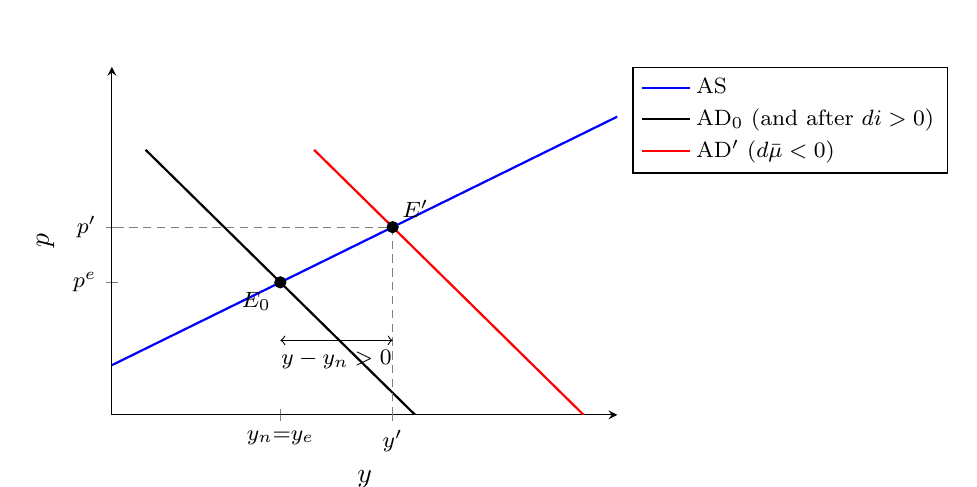
\begin{tikzpicture}
\begin{axis}[width=8cm,height=6cm,xmin=-1,xmax=2,ymin=-0.8,ymax=1.3,axis lines=left,xlabel={$y$},ylabel={$p$},
  xtick={0,0.6667},xticklabels={$y_n{=}y_e$,$y'$},ytick={0,0.3333},yticklabels={$p^e$,$p'$},
  tick label style={font=\footnotesize},legend style={font=\footnotesize},legend pos=outer north east,legend cell align=left]
\addplot[thick,blue,domain=-1:2]{0.5*x};
\addplot[thick,black,domain=-0.8:0.8]{-x};
\addplot[thick,red,domain=0.2:1.8]{-(x-1)};
\legend{AS,AD$_0$ (and after $di>0$),AD$'$ ($d\bar\mu<0$)}
\addplot[only marks,mark=*] coordinates {(0,0) (0.6667,0.3333)};
\node[font=\footnotesize,anchor=north east] at (axis cs:0,0) {$E_0$};
\node[font=\footnotesize,anchor=south west] at (axis cs:0.6667,0.3333) {$E'$};
\draw[gray,densely dashed] (axis cs:0.6667,-0.8) -- (axis cs:0.6667,0.3333) -- (axis cs:-1,0.3333);
\draw[<->] (axis cs:0,-0.35) -- (axis cs:0.6667,-0.35) node[midway,below,font=\footnotesize]{$y-y_n>0$};
\end{axis}
\end{tikzpicture}
\end{center}
{\footnotesize Drawn with $\sigma=1$, $\kappa=0.5$, $d\bar y=1$: $E'=(2/3,1/3)$ (check script). The rise $di=1$ moves AD$'$ back onto AD$_0$.}
\rubrica{
\item Curve and closed forms: 2 pts. Graph (scored on its own): axes, AS through $(y_n,p^e)$, AD$_0$, AD$'$, $E_0$, $E'$, gap: 2 pts.
}
\end{sol}

\textbf{c)} (2 points) In words: what changes if the news is a \emph{rise} in $\bar\mu$ (Prova 01, Q3)? Does the answer depend on $\phi$?
\resolespaco
\begin{sol}
\begin{notacao}
\item Symbols as in (a). Here $d\bar\mu>0$, $d\mu=0$. $\phi\ge0$: the weight on price surprises in the loss \eqref{LF}.
\end{notacao}
\passo{flip}{By \eqref{YB}, $d\bar y=-d\bar\mu/\Omega<0$, so every sign flips: AD left, $y$ and $p$ fall, $y-y_n<0$ and $y-y_e<0$. By \eqref{q2:di}
the bank \textbf{cuts} $i$:}
\begin{align}
di&=\frac{d\bar y}{\sigma}\nonumber\\
&=\frac{(-d\bar\mu/\Omega)}{\sigma}\nonumber\\
&=-\frac{d\bar\mu}{\sigma\Omega}<0 , \nonumber
\end{align}
at no cost. The AS does not move because current $\mu$ did not change. $\phi$ is irrelevant: neither $y_n$ nor $y_e$ moved, so the
optimum of the loss is the old point and the bank only undoes the AD shift (\eqref{q4:di} in Question 4(c)).
\refbib{Benigno (2015), \S6.3, Fig.\ 8, p.~513; \S4.2, p.~508 ($\bar\mu$ in $\bar y$); \texttt{Prova/prova-01-error-analysis.md}, Q3.}
\rubrica{\item AD left and a cut: 1 pt. ``AS moves'' or ``raise $i$'': 0 for the item. $\phi$-independence with the reason: 1 pt.}
\end{sol}

% -----------------------------------------------------------------------------
\questao{(10 points) \textit{Source: MPE Macroeconomics I, Lista 7 (2026), Question 2, item (a) only --- reproduced verbatim (its
points label and item (b) omitted); built also on Benigno, P. (2015), ``New-Keynesian Economics: An AS--AD View'', \S7, Fig.~9,
pp.~513--514, which has no exercises.}}

\noindent\textbf{Lista 7, Question 2.} Using separate AS--AD diagrams, analyze the following changes:
\begin{enumerate}[label=\alph*),leftmargin=2.2em,topsep=2pt,itemsep=1pt]
\item a temporary increase in firms' desired markups;
\end{enumerate}
In each case, identify which curve shifts, indicate the direction of the shift, and describe the effects on output and the price
level. Explain the economic intuition behind the movement of the curve and the resulting equilibrium.

\noindent What Benigno states (p.~513): ``This section considers only temporary mark-up shocks, leaving other analyses to the reader.''

\noindent\textit{Added parts (not in Lista 7), with the sign changed:} the desired markup \emph{falls} for one period only, $d\mu<0$
(a temporary payroll-tax cut, or a fall in the oil price); $d\bar\mu=0$. Items (a)--(c) below are this list's.

\textbf{a)} (3 points) With $i$ fixed: which curve moves and where; $dy$, $dp$, $d(y-y_n)$, $d(y-y_e)$ with signs.
\resolespaco
\begin{sol}
\begin{notacao}
\item $y$, $p$, $\bar y$, $p^e$, $y_n$, $y_e$, $i$, $\mu$, $\bar\mu$, $\sigma>0$, $\kappa>0$, $\Omega\equiv\sigma^{-1}+\eta>0$: as in Question~1.
\item The shock: $d\mu<0$ for one period, $d\bar\mu=0$.
\item $\phi\ge0$: weight on price surprises in \eqref{LF}. $y^*$, $p^*$, $i^*$: the bank's optimal output, price and rate.
\end{notacao}
\passo{curves}{Differentiate \eqref{YN} with only $\mu$ moving:}
\begin{equation}
dy_n=-\frac{d\mu}{\Omega}>0 . \label{q3:dyn}
\end{equation}
\eqref{YE} has no $\mu$, so $dy_e=0$; \eqref{YB} has no current $\mu$, so $d\bar y=0$. The AS shifts \emph{right} (down), through $(y_n',p^e)$;
by \eqref{q1:dAD} the AD stays.
\passo{solution}{Put only $dy_n$ in \eqref{q1:M} and divide by $1+\sigma\kappa$:}
\begin{equation}
d(y-y_n)=\frac{-dy_n}{1+\sigma\kappa}<0 . \label{q3:gap}
\end{equation}
Add $dy_n$ to \eqref{q3:gap}, as in \eqref{q1:dya}:
\begin{align}
dy&=dy_n+\Big(\frac{-dy_n}{1+\sigma\kappa}\Big)\nonumber\\
&=dy_n-\frac{dy_n}{1+\sigma\kappa}\nonumber\\
&=\frac{\sigma\kappa\,dy_n}{1+\sigma\kappa}>0 . \label{q3:dy}
\end{align}
By \eqref{q1:dAS} with $dp^e=0$, $dp=\kappa\,d(y-y_n)$. Substitute \eqref{q3:gap}:
\begin{align}
dp&=\kappa\Big(\frac{-dy_n}{1+\sigma\kappa}\Big)\nonumber\\
&=\frac{-\kappa\,dy_n}{1+\sigma\kappa}<0 . \label{q3:dp}
\end{align}
Since $dy_e=0$, $d(y-y_e)=dy>0$ by \eqref{q3:dy}. The two gaps have \emph{opposite} signs: output is below natural (so prices fall)
and above efficient.
\passo{confirmation}{This is the mirror image of Lista 7, Q2(a). The instructor's key (\texttt{Listas/solu\c{c}\~oes do instrutor/PSET 7 (1).pdf},
p.~1) shifts only the AS, to the left, with the AD fixed and $p'>p^e$; \texttt{Map/lista-07.md} (row 2a) gives $y\downarrow$, $p\uparrow$,
$y-y_n>0$, $y-y_e<0$. Reversing the sign of $d\mu$ reverses every entry, as above.}
\rubrica{\item AS only, right: 1 pt. AD shifted: max.\ 1 pt for the item. \item Closed forms: 1 pt. \item Two gaps with opposite signs: 1 pt; one ``output gap'': 0 for this line.}
\end{sol}

\textbf{b)} (3 points) Find the $di$ that keeps $p=p^e$ and the $di$ that keeps $y=y_e$. Report $y-y_e$ in the first case and $p-p^e$ in
the second. Is there a trade-off?
\resolespaco
\begin{sol}
\begin{notacao}
\item Symbols as in (a).
\end{notacao}
\passo{price stability}{Put $d(y-y_n)=0$ in \eqref{q1:M} with only $di$ and $dy_n$:}
\begin{equation}
0=-\sigma\,di-dy_n . \nonumber
\end{equation}
Solve for $di$ and substitute \eqref{q3:dyn}:
\begin{align}
di&=-\frac{dy_n}{\sigma}\nonumber\\
&=-\frac{(-d\mu/\Omega)}{\sigma}\nonumber\\
&=\frac{d\mu}{\sigma\Omega}<0 , \label{q3:dips}
\end{align}
a cut. Then $dy=dy_n$ and, since $dy_e=0$, $d(y-y_e)=dy_n>0$.
\passo{efficient output}{$y=y_e$ means $dy=0$. Put only $di$ and $dy_n$ in \eqref{q1:dy}:}
\begin{equation}
(1+\sigma\kappa)\,dy=\sigma\kappa\,dy_n-\sigma\,di . \nonumber
\end{equation}
Set $dy=0$ and solve for $di$:
\begin{equation}
di=\kappa\,dy_n>0 , \label{q3:die}
\end{equation}
a rise. By \eqref{q1:dAS} with $dy=0$:
\begin{equation}
dp=\kappa\,(0-dy_n)=-\kappa\,dy_n<0 . \nonumber
\end{equation}
\passo{trade-off}{\eqref{q3:dips} and \eqref{q3:die} have opposite signs: yes, a trade-off. The shock moves $y_n$ and not $y_e$.}
\rubrica{\item Each rate with sign and its outcome: 1 pt each. \item Trade-off traced to $y_n-y_e$: 1 pt.}
\end{sol}

\textbf{c)} (4 points) The bank minimizes $L$. Find $dy^*$, $dp^*$ and $di^*$, and the condition on $\phi$ under which it cuts.
\resolespaco
\begin{sol}
\begin{notacao}
\item Symbols as in (a); $y^*$, $p^*$, $i^*$ and $\phi$ as listed there.
\end{notacao}
\passo{optimum}{Question 4(a) gives the optimum \eqref{q4:ystar}. Differentiate it with $dy_e=0$:}
\begin{equation}
dy^*=\frac{\phi\kappa\,dy_n}{1+\phi\kappa}>0 . \label{q3:dys}
\end{equation}
By \eqref{q1:dAS} with $dp^e=0$, $dp^*=\kappa(dy^*-dy_n)$. Substitute \eqref{q3:dys}:
\begin{align}
dp^*&=\kappa\Big(\frac{\phi\kappa\,dy_n}{1+\phi\kappa}-dy_n\Big)\nonumber\\
&=\kappa\,\frac{\phi\kappa\,dy_n-(1+\phi\kappa)\,dy_n}{1+\phi\kappa}\nonumber\\
&=\frac{-\kappa\,dy_n}{1+\phi\kappa}<0 . \label{q3:dps}
\end{align}
\passo{rate}{Put $d\bar y=dg=d\bar g=d\bar p=0$ in \eqref{q1:dAD}:}
\begin{equation}
dy^*=-\sigma\,di^*-\sigma\,dp^* . \nonumber
\end{equation}
Solve for $di^*$:
\begin{equation}
di^*=-\frac{dy^*+\sigma\,dp^*}{\sigma}. \label{q3:di0}
\end{equation}
Add \eqref{q3:dys} and $\sigma$ times \eqref{q3:dps}:
\begin{align*}
dy^*+\sigma\,dp^*&=\Big(\frac{\phi\kappa\,dy_n}{1+\phi\kappa}\Big)+\sigma\Big(\frac{-\kappa\,dy_n}{1+\phi\kappa}\Big)\\
&=\frac{\phi\kappa\,dy_n-\sigma\kappa\,dy_n}{1+\phi\kappa}\\
&=\frac{\kappa(\phi-\sigma)\,dy_n}{1+\phi\kappa}.
\end{align*}
Substitute this into \eqref{q3:di0}:
\begin{align}
di^*&=-\frac{\Big(\frac{\kappa(\phi-\sigma)\,dy_n}{1+\phi\kappa}\Big)}{\sigma}\nonumber\\
&=-\frac{\kappa(\phi-\sigma)\,dy_n}{\sigma(1+\phi\kappa)}. \label{q3:dis}
\end{align}
\passo{sign}{By \eqref{q3:dyn}, $dy_n>0$. So in \eqref{q3:dis}, $di^*<0$ (cut) iff $\phi>\sigma$, and $di^*>0$ iff $\phi<\sigma$. Compare \eqref{q3:dps}
with the no-policy \eqref{q3:dp}: a hawk ($\phi>\sigma$) wants less price fall than the no-policy point gives
($\frac{1}{1+\phi\kappa}<\frac{1}{1+\sigma\kappa}$), so it pushes AD right.}
\refbib{Benigno (2015), \S7, Fig.\ 9, pp.~513--514; \S11, p.~522 (sign of the response depends on the IT slope); \texttt{Map/benigno/06-markup-shocks.md} \S6.3.}
\rubrica{\item $dy^*$, $dp^*$ from $dL/dy=0$ on AS: 2 pts. Optimisation in $i$ without AS: max.\ 1 pt for the item. \item $di^*$ and the $\phi\gtrless\sigma$ condition: 2 pts.}
\end{sol}

% -----------------------------------------------------------------------------
\questao{(10 points) \emph{Optimal policy.} \textit{Sources: MPE Macroeconomics I, Lista 7 (2026), Question 4 --- reproduced verbatim
(its points label omitted); Carlin, W. and Soskice, D. (2024), \emph{Macroeconomics: Institutions, Instability, and Inequality},
\S3.6.1 checklist questions 4 and 5, p.~156 --- reproduced verbatim; built also on Benigno, P. (2015), ``New-Keynesian Economics:
An AS--AD View'', \S11, eqs.~(33)--(35), Fig.~14, pp.~521--523, which has no exercises.}}

\noindent\textbf{Lista 7, Question 4.} The microeconomic foundations of the New Keynesian model make it possible to evaluate
monetary policy in terms of household welfare.

\noindent Consider the following loss function in conjunction with the AS-AD dynamics seen in Benigno (2015)
\begin{align*}
&\min_{y,p}\mathcal{L}=\phi_y(y-y^*)^2+\phi_p(p-p^e)^2, \qquad \phi_y,\phi_p>0,\\
&\text{s.t:}\\
&p-p^e=\kappa(y-y_n).
\end{align*}
Interpret the shape of the loss function and analyse what it implies for the behavior of a central bank. Also, explain why this
problem is subjected to the AS condition and what does that mean in terms of economic policy

\noindent\textbf{Carlin and Soskice, checklist questions 4 and 5.}
\begin{enumerate}[label=\arabic*.,leftmargin=2.2em,topsep=2pt,itemsep=1pt,start=4]
\item Explain what is meant by the central bank's loss function. How are the central bank's preferences reflected in the loss
function? Draw the loss `circles' for the cases where
\begin{enumerate}[label=(\alph*),topsep=1pt,itemsep=0pt]
\item $\beta=1$;
\item $\beta<1$;
\item $\beta>1$.
\end{enumerate}
In which of the three cases will the central bank reduce inflation back to target quickest after an inflation shock? Is there any
downside to adopting this policy stance?
\item Assume that $\alpha=\beta=1$, derive the $MR$ curve graphically using the tangencies between the loss circles and the Phillips
curves. With reference to the diagrams, explain the effect of the following (in each case, assume all other parameters are held
constant):
\begin{enumerate}[label=(\alph*),topsep=1pt,itemsep=0pt]
\item An increase in the slope of the Phillips curve, $\alpha$
\item An increase in central bank's inflation aversion, $\beta$.
\end{enumerate}
\end{enumerate}

\noindent What Benigno states (p.~522): ``This rule is robust to all types of shock and does not depend on their properties.''

\noindent\textit{Added parts (not in the sources):} items (a)--(c) below are this list's. They ask the questions above in Benigno's
static model and with the loss $L$ of the cover: $\phi$ plays the role of Carlin and Soskice's $\beta$, $\kappa$ of their $\alpha$, the
IT line of their $MR$ curve.

\textbf{a)} (4 points) Minimize $L$ subject to the AS. Derive the targeting rule, explain why the AS (and not the AD) is the constraint,
and describe the loss contours and the IT line. Show that the Lista 7 loss $\phi_y(y-y^*)^2+\phi_p(p-p^e)^2$ gives the same rule for suitable weights.
\resolespaco
\begin{sol}
\begin{notacao}
\item $y$, $p$: log output and price level. $y_n$, $y_e$: natural and efficient output, \eqref{YN} and \eqref{YE}. $p^e$: preset price.
\item $\kappa>0$: slope of \eqref{AS}. $\phi\ge0$: weight on price surprises in the loss $L$ \eqref{LF}. $\sigma>0$, $i$: as in Question~1.
\item $y^*$: the optimal output (in this question). $c>0$: a level of the loss, $L=c$ (a contour).
\item IT line: the targeting rule drawn in the $(y,p)$ plane.
\item Lista 7 loss only: $L_7\equiv\phi_y(y-y^*)^2+\phi_p(p-p^e)^2$; $\phi_y,\phi_p>0$ are its weights and $y^*$ there is that list's output target, not the optimum.
\end{notacao}
\passo{substitution}{Square both sides of \eqref{AS}:}
\begin{equation}
(p-p^e)^2=\kappa^2(y-y_n)^2 . \label{q4:sq}
\end{equation}
Substitute \eqref{q4:sq} into the second term of \eqref{LF}:
\begin{align}
L&=\tfrac12(y-y_e)^2+\tfrac{\phi}{2\kappa}\,\big(\kappa^2(y-y_n)^2\big)\nonumber\\
&=\tfrac12(y-y_e)^2+\tfrac{\phi\kappa}{2}(y-y_n)^2 . \label{q4:Ly}
\end{align}
\passo{FOC}{Differentiate \eqref{q4:Ly} with respect to $y$ and set it to zero:}
\begin{equation}
\frac{dL}{dy}=(y-y_e)+\phi\kappa\,(y-y_n)=0 . \label{q4:foc}
\end{equation}
Differentiate once more: $\frac{d^2L}{dy^2}=1+\phi\kappa>0$, so \eqref{q4:foc} gives a minimum. By \eqref{AS}, $\kappa(y-y_n)=p-p^e$; substitute
this into \eqref{q4:foc}:
\begin{equation}
(y-y_e)+\phi\,(p-p^e)=0 . \label{q4:rule}
\end{equation}
Collect the $y$ terms of \eqref{q4:foc}:
\begin{equation}
y\,(1+\phi\kappa)=y_e+\phi\kappa\,y_n . \nonumber
\end{equation}
Divide by $1+\phi\kappa$:
\begin{equation}
y^*=\frac{y_e+\phi\kappa\,y_n}{1+\phi\kappa}. \label{q4:ystar}
\end{equation}
\passo{why AS}{$i$ enters only \eqref{AD}, and by \eqref{q1:dAD} a change in $i$ shifts the AD horizontally by $-\sigma\,di$: any point of the
AS can be reached. The AD restricts nothing; the AS (firms' price setting) is the menu of $(y,p)$ the bank can choose from.}
\passo{geometry}{Set \eqref{LF} equal to $c$ and divide by $c$:}
\begin{equation}
\frac{(y-y_e)^2}{2c}+\frac{(p-p^e)^2}{2c\kappa/\phi}=1 , \nonumber
\end{equation}
an ellipse centred at $(y_e,p^e)$ (a circle iff $\phi=\kappa$). The optimum is the tangency of the lowest ellipse with the AS. Solve
\eqref{q4:rule} for $p$:
\begin{equation}
p-p^e=-\frac1\phi\,(y-y_e) , \label{q4:IT}
\end{equation}
the IT line: slope $-1/\phi$, through $(y_e,p^e)$.
\passo{Lista 7}{Substitute \eqref{q4:sq} into the Lista 7 loss:}
\begin{equation}
L_7=\phi_y(y-y^*)^2+\phi_p\big(\kappa^2(y-y_n)^2\big) . \nonumber
\end{equation}
Differentiate with respect to $y$, set it to zero and divide by 2:
\begin{equation}
\phi_y(y-y^*)+\phi_p\kappa^2(y-y_n)=0 . \nonumber
\end{equation}
Replace $\kappa(y-y_n)$ by $p-p^e$ using \eqref{AS}:
\begin{equation}
\phi_y(y-y^*)+\kappa\phi_p(p-p^e)=0 , \label{q4:rule7}
\end{equation}
the rule in \texttt{Map/lista-07.md} (Q4). Put $\phi_y=\frac12$, $\phi_p=\frac{\phi}{2\kappa}$, $y^*=y_e$ in \eqref{q4:rule7}:
\begin{align}
\big(\tfrac12\big)\big(y-(y_e)\big)+\kappa\big(\tfrac{\phi}{2\kappa}\big)(p-p^e)&=0\nonumber\\
\tfrac12(y-y_e)+\tfrac\phi2(p-p^e)&=0 , \nonumber
\end{align}
which is \eqref{q4:rule} divided by 2. (The instructor's PSET 7 key does not cover Q4; the check is against the project's verified answer.)
\rubrica{\item Substitution of AS and $dL/dy=0$ with SOC: 2 pts. Differentiating in $i$ or using a $y_e$ that contains $\mu$ (Prova 01, 3.c): max.\ 1 pt.
\item Why AS, contours and IT line: 1.5 pts. \item Lista 7 mapping: 0.5 pt.}
\end{sol}

\textbf{b)} (3 points) Let $W\equiv y_e-y_n>0$. Find $y^*-y_e$ and $p^*-p^e$, sign their derivatives in $\phi$ and $\kappa$, and give the limits
$\phi\to\infty$ and $\phi=0$. Relate the answer to the two Carlin--Soskice questions.
\resolespaco
\begin{sol}
\begin{notacao}
\item Symbols as in (a). New: $W\equiv y_e-y_n>0$, the wedge between efficient and natural output. $p^*$: the optimal price level.
\item $\partial_\phi$, $\partial_\kappa$: partial derivatives with respect to $\phi$ and $\kappa$.
\end{notacao}
\passo{levels}{Subtract $y_n$ from \eqref{q4:ystar}:}
\begin{align}
y^*-y_n&=\frac{y_e+\phi\kappa\,y_n-(1+\phi\kappa)\,y_n}{1+\phi\kappa}\nonumber\\
&=\frac{y_e-y_n}{1+\phi\kappa}\nonumber\\
&=\frac{W}{1+\phi\kappa}. \label{q4:gapn}
\end{align}
Subtract $W=y_e-y_n$ from \eqref{q4:gapn}:
\begin{align}
y^*-y_e&=\frac{W}{1+\phi\kappa}-W\nonumber\\
&=-\frac{\phi\kappa\,W}{1+\phi\kappa}. \label{q4:gape}
\end{align}
By \eqref{AS}, $p^*-p^e=\kappa(y^*-y_n)$. Substitute \eqref{q4:gapn}:
\begin{align}
p^*-p^e&=\kappa\Big(\frac{W}{1+\phi\kappa}\Big)\nonumber\\
&=\frac{\kappa W}{1+\phi\kappa}. \label{q4:pgap}
\end{align}
\passo{derivatives}{Differentiate \eqref{q4:pgap} with respect to $\phi$:}
\begin{equation}
\partial_\phi(p^*-p^e)=-\frac{\kappa^2W}{(1+\phi\kappa)^2}<0 . \nonumber
\end{equation}
Differentiate \eqref{q4:pgap} with respect to $\kappa$ (quotient rule):
\begin{align*}
\partial_\kappa(p^*-p^e)&=\frac{(1+\phi\kappa)-\phi\kappa}{(1+\phi\kappa)^2}\,W\\
&=\frac{W}{(1+\phi\kappa)^2}>0 .
\end{align*}
Differentiate \eqref{q4:gape} with respect to $\phi$ and to $\kappa$:
\begin{align*}
\partial_\phi(y^*-y_e)&=-\frac{\kappa W}{(1+\phi\kappa)^2}<0 ,\\
\partial_\kappa(y^*-y_e)&=-\frac{\phi W}{(1+\phi\kappa)^2}<0 .
\end{align*}
\passo{limits}{Let $\phi\to\infty$ in \eqref{q4:gapn} and \eqref{q4:pgap}: $y^*\to y_n$, $p^*\to p^e$ (strict price stability). Put $\phi=0$ in
\eqref{q4:gape} and \eqref{q4:pgap}: $y^*=y_e$, $p^*-p^e=\kappa W$.}
\passo{Carlin--Soskice}{More inflation aversion ($\phi$, their $\beta$) flattens the IT/MR line \eqref{q4:IT} (slope $-1/\phi$): less of the
wedge into prices, more into output.
A steeper AS ($\kappa$, their $\alpha$) makes each unit of output above $y_n$ cost more price surprise.}
\rubrica{\item Levels: 1 pt. \item Four signed derivatives: 1 pt. \item Limits and the analogy: 1 pt.}
\end{sol}

\textbf{c)} (3 points) For a shock with changes $dy_n$, $dy_e$, $d\bar y$ ($g$, $\bar p$, $p^e$ fixed), find $di^*$ and prove that it depends on $\phi$
if and only if $dy_n\neq dy_e$. Apply the result to news of a higher $\bar\mu$.
\resolespaco
\begin{sol}
\begin{notacao}
\item Symbols as in (a) and (b). $dy_n$, $dy_e$, $d\bar y$: the shock's changes in natural, efficient and long-run output.
\item New: $X\equiv dy_e-dy_n$, the change in the wedge $W$. $i^*$: the optimal rate. $\Omega\equiv\sigma^{-1}+\eta$, $\bar\mu$: as in Question~1.
\end{notacao}
\passo{optimum}{Differentiate \eqref{q4:ystar}:}
\begin{equation}
dy^*=\frac{dy_e+\phi\kappa\,dy_n}{1+\phi\kappa}. \label{q4:dys}
\end{equation}
Write $dy_n=dy_e-X$ in \eqref{q4:dys}:
\begin{align}
dy^*&=\frac{dy_e+\phi\kappa\,(dy_e-X)}{1+\phi\kappa}\nonumber\\
&=\frac{(1+\phi\kappa)\,dy_e-\phi\kappa X}{1+\phi\kappa}\nonumber\\
&=dy_e-\frac{\phi\kappa X}{1+\phi\kappa}. \label{q4:dys2}
\end{align}
By \eqref{q1:dAS} with $dp^e=0$, $dp^*=\kappa(dy^*-dy_n)$. From \eqref{q4:dys}, $dy^*-dy_n=\frac{dy_e-dy_n}{1+\phi\kappa}=\frac{X}{1+\phi\kappa}$, so
\begin{align}
dp^*&=\kappa\Big(\frac{X}{1+\phi\kappa}\Big)\nonumber\\
&=\frac{\kappa X}{1+\phi\kappa}. \label{q4:dps}
\end{align}
\passo{rate}{Put $dg=d\bar g=d\bar p=0$ in \eqref{q1:dAD}:}
\begin{equation}
dy^*=d\bar y-\sigma\,di^*-\sigma\,dp^* . \nonumber
\end{equation}
Solve for $di^*$:
\begin{equation}
di^*=\frac{d\bar y-dy^*-\sigma\,dp^*}{\sigma}. \label{q4:di0}
\end{equation}
Add \eqref{q4:dys2} and $\sigma$ times \eqref{q4:dps}:
\begin{align}
dy^*+\sigma\,dp^*&=\Big(dy_e-\frac{\phi\kappa X}{1+\phi\kappa}\Big)+\sigma\Big(\frac{\kappa X}{1+\phi\kappa}\Big)\nonumber\\
&=dy_e+\frac{(\sigma-\phi)\,\kappa X}{1+\phi\kappa}. \nonumber
\end{align}
Substitute this into \eqref{q4:di0}:
\begin{align}
di^*&=\frac{d\bar y-\Big(dy_e+\frac{(\sigma-\phi)\,\kappa X}{1+\phi\kappa}\Big)}{\sigma}\nonumber\\
&=\frac{d\bar y-dy_e}{\sigma}-\frac{(\sigma-\phi)\,\kappa X}{\sigma(1+\phi\kappa)}. \label{q4:di}
\end{align}
\passo{proof}{Only the last term of \eqref{q4:di} contains $\phi$. Differentiate its $\phi$ part (quotient rule):}
\begin{align*}
\frac{\partial}{\partial\phi}\,\frac{-(\sigma-\phi)}{1+\phi\kappa}&=\frac{(1+\phi\kappa)+(\sigma-\phi)\kappa}{(1+\phi\kappa)^2}\\
&=\frac{1+\sigma\kappa}{(1+\phi\kappa)^2}.
\end{align*}
Multiply by $\frac{\kappa X}{\sigma}$:
\begin{equation}
\frac{\partial di^*}{\partial\phi}=\frac{\kappa(1+\sigma\kappa)\,X}{\sigma(1+\phi\kappa)^2}, \label{q4:ddi}
\end{equation}
zero iff $X=0$. With $X=0$, $dy_e=dy_n$; substitute both into \eqref{q4:di}:
\begin{align}
di^*&=\frac{d\bar y-(dy_n)}{\sigma}-\frac{(\sigma-\phi)\,\kappa\,(0)}{\sigma(1+\phi\kappa)}\nonumber\\
&=\frac{d\bar y-dy_n}{\sigma}, \nonumber
\end{align}
the strict price-stability rate (\eqref{q1:M} with $d(y-y_n)=0$).
\passo{$\bar\mu$ news}{By \eqref{YN} and \eqref{YE}, $dy_n=dy_e=0$, so $X=0$; by \eqref{YB}, $d\bar y=-\frac{d\bar\mu}{\Omega}$. Substitute into \eqref{q4:di}:}
\begin{align}
di^*&=\frac{(-d\bar\mu/\Omega)-(0)}{\sigma}-\frac{(\sigma-\phi)\,\kappa\,(0)}{\sigma(1+\phi\kappa)}\nonumber\\
&=-\frac{d\bar\mu}{\sigma\Omega}<0 \nonumber
\end{align}
for every $\phi$, as in Prova 01, 3.c (error analysis, Q3).
\intuicao{$\phi$ chooses a point on the AS only when the shock separates $y_n$ from $y_e$; otherwise the best point is unique and the
bank just moves AD back to it.}
\rubrica{\item $di^*$ in closed form: 1.5 pts. \item Proof of the iff: 1 pt. \item Application, with ``cut, for any $\phi$'': 0.5 pt.}
\end{sol}

% =============================================================================
\bloco{2}{Harder and conceptual: which bar moves which curve, signs, divine coincidence, zero bound}{Benigno \S\S4--11 \,\textbullet\, 38 points}

\questao{(10 points) \emph{Which bar moves which curve.} Consider a small rise, one at a time, in each of $a,\bar a,\mu,\bar\mu,g,\bar g,\bar p,p^e$.}

\textbf{a)} (6 points) Build a table with, for each variable: the curve that moves and its shift (horizontal for AD and AS; vertical for
$p^e$); whether $y_e$ moves; whether there is a trade-off; and the $di$ (sign and closed form) that keeps $y=y_n$ and $p=p^e$.
\resolespaco
\begin{sol}
\begin{notacao}
\item $y$, $p$, $\bar y$, $\bar p$, $p^e$, $y_n$, $y_e$, $i$, $a$, $\bar a$, $\mu$, $\bar\mu$, $g$, $\bar g$, $\sigma>0$, $\eta>0$, $\kappa>0$, $\Omega\equiv\sigma^{-1}+\eta$: as in
Question~1. Each row is a small rise $d(\cdot)>0$ in one variable, the others fixed; $\bar p$ and $p^e$ move only in their own rows.
\item Trade-off: price stability and $y=y_e$ cannot both be reached with $i$.
\end{notacao}
\passo{method}{By \eqref{q1:dAS} the AS shifts horizontally by $dy_n$ (or vertically by $dp^e$); by \eqref{q1:dAD} the AD shifts horizontally by
$d\bar y+dg-d\bar g+\sigma\,d\bar p$. $y=y_n$ and $p=p^e$ mean $d(y-y_n)=0$; put this in \eqref{q1:M} of Question~1:}
\begin{equation}
0=d\bar y+dg-d\bar g-\sigma\,di+\sigma(d\bar p-dp^e)-dy_n . \nonumber
\end{equation}
Solve for $di$:
\begin{equation}
di=\frac{d\bar y+dg-d\bar g-dy_n}{\sigma}+d\bar p-dp^e . \label{q5:di}
\end{equation}
Each row fills \eqref{q5:di} with the derivatives of \eqref{YN} and \eqref{YB}; $y_e$ moves by the derivative of \eqref{YE}.
\begin{center}\small
\begin{tabular}{lllccl}
\toprule
Rise in & Curve that moves (shift) & Through & $y_e$ moves? & Trade-off? & $di$ for $p=p^e$ \\
\midrule
$a$ & AS right, $\frac{1+\eta}{\Omega}da$ & $y_n$ & yes, equally & no & $-\frac{(1+\eta)da}{\sigma\Omega}$ (cut) \\
$\bar a$ & AD right, $\frac{1+\eta}{\Omega}d\bar a$ & $\bar y$ & no & no & $+\frac{(1+\eta)d\bar a}{\sigma\Omega}$ (raise) \\
$\mu$ & AS left, $\frac{1}{\Omega}d\mu$ & $y_n$ & \textbf{no} & \textbf{yes} & $+\frac{d\mu}{\sigma\Omega}$ (raise) \\
$\bar\mu$ & AD left, $\frac{1}{\Omega}d\bar\mu$ & $\bar y$ & no & no & $-\frac{d\bar\mu}{\sigma\Omega}$ (cut) \\
$g$ & AD right $dg$; AS right $\frac{\sigma^{-1}}{\Omega}dg$ & both & yes, equally & no & $+\frac{\eta\,dg}{\sigma\Omega}$ (raise) \\
$\bar g$ & AD left, $\frac{\eta}{\Omega}d\bar g$ & $\bar y-\bar g$ & no & no & $-\frac{\eta\,d\bar g}{\sigma\Omega}$ (cut) \\
$\bar p$ & AD right, $\sigma\,d\bar p$ & $\bar p-p$ & no & no & $+d\bar p$ (raise) \\
$p^e$ & AS up, $dp^e$ (vertical) & $p^e$ & no & no & $-dp^e$ (cut) \\
\bottomrule
\end{tabular}
\end{center}
\passo{the two subtle rows}{$\bar g$: by \eqref{YB}, $d\bar y=\frac{\sigma^{-1}}{\Omega}d\bar g$. The AD shift is then}
\begin{align}
d\bar y-d\bar g&=\Big(\frac{\sigma^{-1}}{\Omega}\,d\bar g\Big)-d\bar g\nonumber\\
&=\Big(\frac{\sigma^{-1}}{\Omega}-1\Big)d\bar g\nonumber\\
&=\frac{\sigma^{-1}-\sigma^{-1}-\eta}{\Omega}\,d\bar g\nonumber\\
&=-\frac{\eta}{\Omega}\,d\bar g \label{q5:gb}
\end{align}
(long-run consumption falls); \eqref{q5:di} gives $di=-\frac{\eta\,d\bar g}{\sigma\Omega}$. $g$: by \eqref{YN}, $dy_n=\frac{\sigma^{-1}}{\Omega}dg$, so the gap pressure
in \eqref{q5:di} is
\begin{align}
dg-dy_n&=dg-\Big(\frac{\sigma^{-1}}{\Omega}\,dg\Big)\nonumber\\
&=\frac{\eta}{\Omega}\,dg , \nonumber
\end{align}
by the same step as \eqref{q5:gb}. $p^e$: with $p^e$ higher and $\bar p$ fixed, $p=p^e$ means lower expected inflation $\bar p-p$, so a
higher real rate; by \eqref{q5:di}, $i$ must fall one for one.
\rubrica{\item One point per correct pair of rows (curve, shift, $y_e$, trade-off, $di$), up to 6. A row with the wrong curve: 0 for that row.}
\end{sol}

\textbf{b)} (2 points) In words: state the rule that tells you which curve a variable moves.
\resolespaco
\begin{sol}
\begin{notacao}
\item Symbols as in (a). Euler equation: the household's condition linking consumption today to expected long-run consumption.
\end{notacao}
\passo{rule}{Current real fundamentals ($a$, $\mu$, $g$) change what firms can produce at stable prices today, so they move $y_n$ and the AS.
Long-run fundamentals ($\bar a$, $\bar\mu$, $\bar g$) change long-run consumption, which reaches today only through the Euler equation, so they
move the AD. $g$ is also spending today, so it moves both. Nominal anchors: $\bar p$ moves the AD (expected inflation), $p^e$ the AS.}
\rubrica{\item Rule with the Euler channel for the bars: 2 pts; a list without the reason: 1 pt.}
\end{sol}

\textbf{c)} (2 points) In words: why is $\mu$ the only row with a trade-off?
\resolespaco
\begin{sol}
\begin{notacao}
\item Symbols as in (a).
\end{notacao}
\passo{reason}{Subtract \eqref{YE} from \eqref{YN}:}
\begin{equation}
y_n-y_e=-\frac{\mu}{\Omega}. \label{q5:wedge}
\end{equation}
A trade-off exists iff the shock moves \eqref{q5:wedge}. Only current $\mu$ enters $y_n$ without entering $y_e$: the planner
does not face the markup. The bars are long-run variables, and the short-run gap between $y_n$ and $y_e$ does not contain them.
\refbib{Benigno (2015), \S4.1--\S4.4, eqs.\ (15), (19), (21), pp.~507--509; \S\S6--8, pp.~511--517; Kurlat (2020), \S11.2, p.~208 (Fisher equation, row $\bar p$).}
\rubrica{\item The criterion $d(y_n-y_e)\neq0$: 1 pt. \item Why the bars do not enter it: 1 pt.}
\end{sol}

% -----------------------------------------------------------------------------
\questao{(8 points) \emph{Diagnose the answer (words only, no algebra).} News arrives that the long-run markup will rise ($d\bar\mu>0$;
current $\mu$ unchanged). A student writes four claims. For each, say whether it is right and, if not, correct it in words.}
\begin{enumerate}[label=(\arabic*),leftmargin=2em]
\item ``Firms will charge higher markups, so the AS shifts left.''
\item ``Along the AD, prices go up and output goes down.''
\item ``To keep prices stable the bank must raise $i$, accepting a deeper recession as the price of stable prices.''
\item ``The optimal response depends on whether $\phi$ is larger than $\sigma$, i.e.\ on whether the IT line is flatter than the AD.''
\end{enumerate}
\resolespaco
\begin{sol}
\begin{notacao}
\item $\mu$, $\bar\mu$: current and long-run markup; here $d\bar\mu>0$, $d\mu=0$. $y$, $p$, $\bar y$, $p^e$, $y_n$, $y_e$, $i$: as in Question~1.
\item $\phi\ge0$: weight on price surprises in \eqref{LF}; $\sigma>0$: intertemporal elasticity (the slope of AD is $-1/\sigma$ in $(y,p)$).
\end{notacao}
\passo{(1) wrong}{Today's prices are set with today's markup $\mu$, which has not changed; by \eqref{YN}, $y_n$ and the AS do not move. By
\eqref{YB} the news lowers long-run output $\bar y$, hence expected long-run consumption; consumption smoothing cuts spending today: the \textbf{AD} shifts left.}
\passo{(2) wrong}{``$p$ up, $y$ down'' is the signature of an AS shift, which did not happen. The AD moves left along a fixed AS, so the new
point has \emph{both} lower output and lower prices: a demand-driven recession, $y-y_n<0$ and $y-y_e<0$.}
\passo{(3) wrong sign, wrong cost}{Prices are below $p^e$; to restore them the bank must bring the AD back to the right: \textbf{cut} $i$. A rise
deepens both the fall in prices and the recession. The cut has no cost: it returns the economy to the initial point, where both gaps are
zero (a pure AD shock; divine coincidence).}
\passo{(4) wrong}{$\phi$ chooses a point on the AS only when the shock separates $y_n$ from $y_e$ (\eqref{q4:ddi}, Question 4(c)). Here neither
moves, so the best point is the old one for every $\phi$, and the bank fully offsets the AD shift. ($\phi\gtrless\sigma$ decides the sign only for a current markup
shock, Question 3(c).)}
\refbib{\texttt{Prova/prova-01-error-analysis.md}, Q3 and error cluster 5; Benigno (2015), \S6.3, p.~513; \S11, pp.~521--523.}
\rubrica{\item 2 pts per claim: 0.5 for the verdict, 1.5 for the correction with its mechanism. A verdict without a reason: 0.5 at most.}
\end{sol}

% -----------------------------------------------------------------------------
\questao{(9 points) \emph{When does the divine coincidence fail?} True or false; justify each in words (1.5 points each).}
\par\smallskip\noindent\fbox{\parbox{\dimexpr\linewidth-2\fboxsep-2\fboxrule}{\small\textbf{Context from the source (added by this list, from
Benigno 2015, pp.~507--509, 513--514 and 522):} For (a): in the model only prices are sticky (a fraction of firms presets $p^e$);
``An important assumption here is that of wage flexibility.'' (fn.~9, p.~513). For (c): the loss (33) of Question~4 is a second-order
approximation of utility, and ``The approximation holds around an efficient steady state in which $\mu=0$.'' (fn.~21, p.~522). For (d):
the consumption-tax rate $\tau_c$ (with $\tau_l$, $\tau_w$, $\tau_y$ the tax rates on labour income, labour costs and sales) enters the
aggregate markup, $\mu\approx\mu_\theta+\tau_l+\tau_w+\tau_y+\tau_c$ (p.~514), hence (YN), Benigno (15); and it enters the AD, (21), p.~509:
\[ y=\bar y_n+(g-\bar g)-\sigma[i-(\bar p-p)-(\bar\tau_c-\tau_c)-\rho] . \]
(YE), Benigno (19), p.~509, contains no tax rate.}}\par\smallskip

\textbf{a)} If nominal wages were preset as well as prices, a productivity shock could create a trade-off between price stability and
the efficient output gap.
\gabarito{T}
\begin{sol}
\begin{notacao}
\item $y_n$, $y_e$: natural and efficient output, \eqref{YN} and \eqref{YE}; trade-off as in Question~5. $g$, $\mu$, $\bar a$, $\bar\mu$, $i$:
as in Question~1; $\Omega\equiv\sigma^{-1}+\eta$, $\sigma,\eta>0$. $\phi\ge0$: weight in \eqref{LF}. These symbols serve all six items.
\end{notacao}
\passo{reason}{The no-trade-off result for productivity rests on flexible wages: they make $y_n$ move one for one with $y_e$. With preset wages
the real wage cannot follow productivity, and $y_n$ and $y_e$ separate (Benigno fn.~9, p.~513).}
\end{sol}

\textbf{b)} A temporary rise in $g$ forces the bank to choose between stable prices and a zero efficient gap.
\gabarito{F}
\begin{sol}
\passo{reason}{Differentiating \eqref{YN} and \eqref{YE}, $g$ moves $y_n$ and $y_e$ by the same $\frac{\sigma^{-1}}{\Omega}dg$. Raising $i$ to put $y$ at $y_n$ also puts it at $y_e$: one instrument, one target.}
\end{sol}

\textbf{c)} Around a steady state with a large markup distortion, $y_e$ need not be the welfare-relevant target, and the results for
markup shocks are the ones most at risk.
\gabarito{T}
\begin{sol}
\passo{reason}{The quadratic loss is an approximation around an efficient steady state; in the distorted case the target changes and the
optimal response to markup shocks is what changes most (Benigno fn.~21, p.~522).}
\end{sol}

\textbf{d)} A temporary rise in the consumption tax is a pure demand shock, so it creates no trade-off.
\gabarito{F}
\begin{sol}
\passo{reason}{It raises the effective markup (AS left, $y_n$ falls, $y_e$ does not) \emph{and} changes the intertemporal price of consumption
(AD). The markup part separates $y_n$ from $y_e$: a trade-off (Benigno \S8, p.~515).}
\end{sol}

\textbf{e)} After bad news about $\bar a$, if the zero bound binds, the bank faces a trade-off between price stability and the efficient gap.
\gabarito{F}
\begin{sol}
\passo{reason}{Both targets ask for the same thing: more demand, since prices and output are both too low. The zero bound limits the
instrument; it does not make the targets conflict. The coincidence holds; it just cannot be implemented with $i$ alone.}
\end{sol}

\textbf{f)} A dovish bank ($\phi<\sigma$) answers news of a higher $\bar\mu$ with a larger cut than a hawkish bank.
\gabarito{F}
\begin{sol}
\passo{reason}{The cut is $\frac{d\bar\mu}{\sigma\Omega}$ for every $\phi$ (\eqref{q4:di} with $X=0$, Question 4(c)): the news moves neither $y_n$ nor $y_e$.}
\rubrica{\item Each item: 0.5 for the verdict, 1 for the justification. A verdict without a justification: 0.5 at most (T/F rule of the cover applies to the verdicts).}
\end{sol}

% -----------------------------------------------------------------------------
\questao{(11 points) \emph{The zero bound after $\bar\mu$ news.} Start from the steady state with $i=\rho>0$. News arrives that the long-run
markup will rise, $d\bar\mu>0$; current $\mu$ is unchanged and the bank cannot set $i<0$.}

\textbf{a)} (3 points) Find the rate that keeps $p=p^e$ and the size $d\bar\mu^*$ above which the zero bound binds. Interpret with the natural rate.
\resolespaco
\begin{sol}
\begin{notacao}
\item $y$, $p$, $\bar y$, $\bar p$, $p^e$, $y_n$, $y_e$, $i$, $\mu$, $\bar\mu$, $g$, $\sigma>0$, $\eta>0$, $\kappa>0$, $\Omega\equiv\sigma^{-1}+\eta$: as in Question~1.
\item $\rho\equiv-\ln\beta>0$: the initial rate, $i=\rho$ (at the steady state \eqref{AD} holds with $y=\bar y$, $p=\bar p$, $g=\bar g$). The zero bound: $i\ge0$.
\item The shock: $d\bar\mu>0$, $d\mu=0$. $d\bar\mu^*>0$: the size at which the zero bound starts to bind.
\item $r_n\equiv\rho+\sigma^{-1}(\bar y-y_n)$: the natural real interest rate.
\end{notacao}
\passo{rate}{By \eqref{YB}, $d\bar y=-\frac{d\bar\mu}{\Omega}$; by \eqref{YN}, $dy_n=0$. Put $d(y-y_n)=0$ in \eqref{q1:M}:}
\begin{equation}
0=d\bar y-\sigma\,di . \nonumber
\end{equation}
Solve for $di$ and substitute $d\bar y$:
\begin{align}
di&=\frac{d\bar y}{\sigma}\nonumber\\
&=\frac{(-d\bar\mu/\Omega)}{\sigma}\nonumber\\
&=-\frac{d\bar\mu}{\sigma\Omega}. \label{q8:di}
\end{align}
Add \eqref{q8:di} to the initial $i=\rho$:
\begin{align}
i&=\rho+\Big(-\frac{d\bar\mu}{\sigma\Omega}\Big)\nonumber\\
&=\rho-\frac{d\bar\mu}{\sigma\Omega}. \label{q8:i}
\end{align}
\passo{threshold}{The rate \eqref{q8:i} is negative iff}
\begin{equation}
\frac{d\bar\mu}{\sigma\Omega}>\rho . \nonumber
\end{equation}
Multiply by $\sigma\Omega>0$:
\begin{equation}
d\bar\mu>d\bar\mu^*\equiv\sigma\Omega\rho . \label{q8:thr}
\end{equation}
\passo{reading}{Initially $\bar y=y_n$, so $r_n=\rho$. After the news, $dr_n=\sigma^{-1}d\bar y$; substitute $d\bar y$ from \eqref{YB} into $r_n=\rho+dr_n$:}
\begin{align}
r_n&=\rho+\sigma^{-1}\Big(-\frac{d\bar\mu}{\Omega}\Big)\nonumber\\
&=\rho-\frac{d\bar\mu}{\sigma\Omega} , \nonumber
\end{align}
the rate \eqref{q8:i} is the natural rate. Bad enough news makes it negative, and no nominal $i\ge0$ reaches it.
\rubrica{\item Rate: 1.5 pts. Threshold: 1 pt. Natural-rate reading: 0.5 pt.}
\end{sol}

\textbf{b)} (3 points) Let $d\bar\mu>d\bar\mu^*$ and $i=0$. Find $dy$, $dp$, $d(y-y_n)$, $d(y-y_e)$. Is there a trade-off?
\resolespaco
\begin{sol}
\begin{notacao}
\item Symbols as in (a); here $d\bar\mu>d\bar\mu^*$.
\end{notacao}
\passo{solution}{Going from $i=\rho$ to $i=0$ is $di=-\rho$. Put this and $d\bar y=-\frac{d\bar\mu}{\Omega}$ in \eqref{q1:M}:}
\begin{align}
(1+\sigma\kappa)\,d(y-y_n)&=\Big(-\frac{d\bar\mu}{\Omega}\Big)-\sigma(-\rho)\nonumber\\
&=-\frac{d\bar\mu}{\Omega}+\sigma\rho . \nonumber
\end{align}
Divide by $1+\sigma\kappa$; as $dy_n=dy_e=0$, output and both gaps move together:
\begin{equation}
dy=d(y-y_n)=d(y-y_e)=\frac{\sigma\rho-d\bar\mu/\Omega}{1+\sigma\kappa}<0 , \label{q8:dy}
\end{equation}
negative because \eqref{q8:thr} gives $d\bar\mu/\Omega>\sigma\rho$. By \eqref{q1:dAS}, $dp=\kappa\,dy$; substitute \eqref{q8:dy}:
\begin{align}
dp&=\kappa\Big(\frac{\sigma\rho-d\bar\mu/\Omega}{1+\sigma\kappa}\Big)\nonumber\\
&=\frac{\kappa(\sigma\rho-d\bar\mu/\Omega)}{1+\sigma\kappa}<0 . \nonumber
\end{align}
\passo{trade-off}{No: both prices and output are too low; the bank lacks the instrument, not a compatible target (Question 7(e)).}
\rubrica{\item Closed forms: 2 pts. \item No trade-off, with the reason: 1 pt.}
\end{sol}

\textbf{c)} (3 points) Find the commitment $d\bar p$ that restores $y=y_n$ and $p=p^e$ with $i=0$. Explain the channel and why credibility matters.
\resolespaco
\begin{sol}
\begin{notacao}
\item Symbols as in (a). $d\bar p$: the promised change in the long-run price level. $\bar p-p$: expected inflation; $i-(\bar p-p)$: the real rate.
\end{notacao}
\passo{size}{Put $d(y-y_n)=0$, $di=-\rho$, $d\bar y=-\frac{d\bar\mu}{\Omega}$ and $d\bar p$ in \eqref{q1:M}:}
\begin{align}
0&=\Big(-\frac{d\bar\mu}{\Omega}\Big)-\sigma(-\rho)+\sigma\,d\bar p\nonumber\\
&=-\frac{d\bar\mu}{\Omega}+\sigma\rho+\sigma\,d\bar p . \nonumber
\end{align}
Solve for $d\bar p$:
\begin{equation}
d\bar p=\frac{d\bar\mu}{\sigma\Omega}-\rho>0 , \label{q8:pb}
\end{equation}
positive by \eqref{q8:thr}.
\passo{channel}{A higher long-run price level raises expected inflation $\bar p-p$, so the real rate $i-(\bar p-p)$ falls with $i$ stuck at 0
(Fisher equation; long-run neutrality makes $\bar p$ costless for $\bar y$).}
\passo{credibility}{Next period the bank would prefer not to deliver the higher $\bar p$; if households expect it to renege, $\bar p$ does not move
and neither does the AD.}
\refbib{Benigno (2015), \S9, pp.~517--519; Kurlat (2020), \S11.2, p.~208.}
\rubrica{\item $d\bar p$: 1.5 pts. \item Channel: 1 pt. \item Credibility: 0.5 pt.}
\end{sol}

\textbf{d)} (2 points) Alternatively, find the temporary $dg$ that restores $p=p^e$ at $i=0$, and say why fiscal policy works here.
\resolespaco
\begin{sol}
\begin{notacao}
\item Symbols as in (a). $dg$: the temporary rise in public spending ($d\bar g=0$).
\end{notacao}
\passo{size}{Differentiate \eqref{YN} with only $g$ moving:}
\begin{equation}
dy_n=\frac{\sigma^{-1}}{\Omega}\,dg . \label{q8:dyn}
\end{equation}
Put $d(y-y_n)=0$, $di=-\rho$, $d\bar y=-\frac{d\bar\mu}{\Omega}$, $dg$ and \eqref{q8:dyn} in \eqref{q1:M}:
\begin{align}
0&=\Big(-\frac{d\bar\mu}{\Omega}\Big)+dg-\sigma(-\rho)-\Big(\frac{\sigma^{-1}}{\Omega}\,dg\Big)\nonumber\\
&=-\frac{d\bar\mu}{\Omega}+\sigma\rho+dg-\frac{\sigma^{-1}}{\Omega}\,dg . \nonumber
\end{align}
Use $1-\frac{\sigma^{-1}}{\Omega}=\frac{\eta}{\Omega}$ (as in \eqref{q5:gb}):
\begin{equation}
0=-\frac{d\bar\mu}{\Omega}+\sigma\rho+\Big(\frac{\eta}{\Omega}\Big)dg . \nonumber
\end{equation}
Move the other terms to the left side:
\begin{equation}
\frac{\eta}{\Omega}\,dg=\frac{d\bar\mu}{\Omega}-\sigma\rho . \nonumber
\end{equation}
Multiply by $\Omega/\eta$:
\begin{equation}
dg=\frac{d\bar\mu-\sigma\Omega\rho}{\eta}>0 , \label{q8:g}
\end{equation}
positive by \eqref{q8:thr}.
\passo{why}{By \eqref{q1:dAD} $g$ shifts the AD by $dg$, and by \eqref{q8:dyn} the AS only by $\frac{\sigma^{-1}}{\Omega}dg$, so it closes the gap; with $i$ stuck, there is no rate rise to crowd it out.}
\refbib{Benigno (2015), \S8, pp.~514--517; \S9, pp.~517--519.}
\rubrica{\item $dg$: 1.5 pts. \item Reason: 0.5 pt.}
\end{sol}

% =============================================================================
\bloco{3}{Created items: two shocks at once, and the timing of fiscal news}{created \,\textbullet\, 22 points}

\questao{(12 points) \emph{Created.} An oil-price rise lifts the current markup, $d\mu>0$, and in the same week a law is passed that raises
a payroll tax from next period on, $d\bar\mu>0$. The bank minimizes $L$ with a general $\phi\ge0$.}

\textbf{a)} (3 points) With $i$ fixed: which curves move? Find $dy$, $dp$, $d(y-y_n)$, $d(y-y_e)$. When do prices rise?
\resolespaco
\begin{sol}
\begin{notacao}
\item $y$, $p$, $\bar y$, $p^e$, $y_n$, $y_e$, $i$, $\sigma>0$, $\eta>0$, $\kappa>0$, $\Omega\equiv\sigma^{-1}+\eta$: as in Question~1.
\item The shocks: $d\mu>0$ (current markup) and $d\bar\mu>0$ (long-run markup), at the same time.
\item $\phi\ge0$: weight on price surprises in \eqref{LF}. $y^*$, $p^*$, $i^*$: optimal output, price and rate.
\end{notacao}
\passo{curves}{Differentiate \eqref{YN}, \eqref{YB} and \eqref{YE}:}
\begin{equation}
dy_n=-\frac{d\mu}{\Omega},\qquad d\bar y=-\frac{d\bar\mu}{\Omega},\qquad dy_e=0 . \label{q9:shifts}
\end{equation}
So the AS shifts left (by $|dy_n|$) and, by \eqref{q1:dAD}, the AD shifts left (by $|d\bar y|$).
\passo{solution}{Put \eqref{q9:shifts} in \eqref{q1:M} with $di=0$:}
\begin{align}
(1+\sigma\kappa)\,d(y-y_n)&=\Big(-\frac{d\bar\mu}{\Omega}\Big)-\Big(-\frac{d\mu}{\Omega}\Big)\nonumber\\
&=-\frac{d\bar\mu}{\Omega}+\frac{d\mu}{\Omega} . \nonumber
\end{align}
Divide by $1+\sigma\kappa$:
\begin{equation}
d(y-y_n)=\frac{d\mu-d\bar\mu}{\Omega(1+\sigma\kappa)} . \label{q9:gap}
\end{equation}
By \eqref{q1:dAS}, $dp=\kappa\,d(y-y_n)$; substitute \eqref{q9:gap}:
\begin{align}
dp&=\kappa\Big(\frac{d\mu-d\bar\mu}{\Omega(1+\sigma\kappa)}\Big)\nonumber\\
&=\frac{\kappa(d\mu-d\bar\mu)}{\Omega(1+\sigma\kappa)} . \label{q9:dp}
\end{align}
Output is $dy=dy_n+d(y-y_n)$; substitute \eqref{q9:shifts} and \eqref{q9:gap}:
\begin{align}
dy&=\Big(-\frac{d\mu}{\Omega}\Big)+\Big(\frac{d\mu-d\bar\mu}{\Omega(1+\sigma\kappa)}\Big)\nonumber\\
&=-\frac{d\mu}{\Omega}+\frac{d\mu-d\bar\mu}{\Omega(1+\sigma\kappa)}\nonumber\\
&=\frac{-(1+\sigma\kappa)\,d\mu+d\mu-d\bar\mu}{\Omega(1+\sigma\kappa)}\nonumber\\
&=-\frac{\sigma\kappa\,d\mu+d\bar\mu}{\Omega(1+\sigma\kappa)}<0 . \label{q9:dy}
\end{align}
Since $dy_e=0$, $d(y-y_e)=dy<0$.
\passo{prices}{By \eqref{q9:dp}, $dp>0$ iff $d\mu>d\bar\mu$: the supply shift dominates the demand shift.}
\rubrica{\item Both curves, each with its reason: 1 pt. Only one curve moved: max.\ 1 pt for the item. \item Closed forms: 1.5 pts. \item Price condition: 0.5 pt.}
\end{sol}

\textbf{b)} (4 points) Find $dy^*$, $dp^*$, $di^*$ under the optimal rule. Split $di^*$ into a part due to $d\bar\mu$ and a part due to $d\mu$; show
which depends on $\phi$; sign $\partial di^*/\partial\phi$; give the limits $\phi\to\infty$ and $\phi=0$, and the condition for a cut.
\resolespaco
\begin{sol}
\begin{notacao}
\item Symbols as in (a). $X\equiv dy_e-dy_n$: change in the wedge, as in Question 4(c).
\end{notacao}
\passo{optimum}{By \eqref{q9:shifts}, $dy_e=0$ and $X=-dy_n=\frac{d\mu}{\Omega}$. Put these in \eqref{q4:dys}:}
\begin{align}
dy^*&=\frac{\phi\kappa\,dy_n}{1+\phi\kappa}\nonumber\\
&=\frac{\phi\kappa\,(-d\mu/\Omega)}{1+\phi\kappa}\nonumber\\
&=-\frac{\phi\kappa\,d\mu}{\Omega(1+\phi\kappa)} . \label{q9:dys}
\end{align}
Put $X=\frac{d\mu}{\Omega}$ in \eqref{q4:dps}:
\begin{align}
dp^*&=\frac{\kappa\,(d\mu/\Omega)}{1+\phi\kappa}\nonumber\\
&=\frac{\kappa\,d\mu}{\Omega(1+\phi\kappa)} . \label{q9:dps}
\end{align}
$d\bar\mu$ is absent from both.
\passo{rate}{Put $dy_e=0$ and $X=\frac{d\mu}{\Omega}$ in \eqref{q4:di}:}
\begin{align}
di^*&=\frac{d\bar y}{\sigma}-\frac{(\sigma-\phi)\,\kappa\,(d\mu/\Omega)}{\sigma(1+\phi\kappa)}\nonumber\\
&=\frac{d\bar y}{\sigma}-\frac{(\sigma-\phi)\,\kappa\,d\mu}{\sigma\Omega(1+\phi\kappa)} . \nonumber
\end{align}
Substitute $d\bar y$ from \eqref{q9:shifts}:
\begin{align}
di^*&=\frac{(-d\bar\mu/\Omega)}{\sigma}-\frac{(\sigma-\phi)\,\kappa\,d\mu}{\sigma\Omega(1+\phi\kappa)}\nonumber\\
&=\underbrace{-\frac{d\bar\mu}{\sigma\Omega}}_{\text{news: cut, any }\phi}+\underbrace{\frac{\kappa(\phi-\sigma)\,d\mu}{\sigma\Omega(1+\phi\kappa)}}_{\text{current shock: sign of }\phi-\sigma}. \label{q9:di}
\end{align}
\passo{$\phi$}{Put $X=\frac{d\mu}{\Omega}$ in \eqref{q4:ddi}:}
\begin{align}
\frac{\partial di^*}{\partial\phi}&=\frac{\kappa(1+\sigma\kappa)\,(d\mu/\Omega)}{\sigma(1+\phi\kappa)^2}\nonumber\\
&=\frac{\kappa(1+\sigma\kappa)\,d\mu}{\sigma\Omega(1+\phi\kappa)^2}>0 . \nonumber
\end{align}
Limits: as $\phi\to\infty$, $\frac{\phi-\sigma}{1+\phi\kappa}\to\frac1\kappa$, so \eqref{q9:di} tends to
\begin{align}
di^*&\to-\frac{d\bar\mu}{\sigma\Omega}+\Big(\frac1\kappa\Big)\frac{\kappa\,d\mu}{\sigma\Omega}\nonumber\\
&=\frac{d\mu-d\bar\mu}{\sigma\Omega} , \nonumber
\end{align}
strict price stability (equal to \eqref{q1:M} with $d(y-y_n)=0$). At $\phi=0$, $\frac{\kappa(\phi-\sigma)}{\sigma(1+\phi\kappa)}=-\kappa$, so \eqref{q9:di} gives
\begin{align}
di^*&=-\frac{d\bar\mu}{\sigma\Omega}+(-\kappa)\frac{d\mu}{\Omega}\nonumber\\
&=-\frac{d\bar\mu}{\sigma\Omega}-\frac{\kappa\,d\mu}{\Omega} . \nonumber
\end{align}
\passo{cut}{By \eqref{q9:di}, $di^*<0$ iff}
\begin{equation}
\frac{d\bar\mu}{\sigma\Omega}>\frac{\kappa(\phi-\sigma)\,d\mu}{\sigma\Omega(1+\phi\kappa)} . \nonumber
\end{equation}
Multiply by $\sigma\Omega>0$:
\begin{equation}
d\bar\mu>\frac{\kappa(\phi-\sigma)}{1+\phi\kappa}\,d\mu , \label{q9:cut}
\end{equation}
always true if $\phi\le\sigma$ (the right side is then $\le0$).
\intuicao{Contrast with Prova 01: there only the news part existed, so $\phi$ did not matter. Here $\phi$ matters, but only through the current
markup, the one shock that separates $y_n$ from $y_e$.}
\rubrica{\item $dy^*$, $dp^*$ from the rule on AS: 1 pt. \item $di^*$ and its split: 1.5 pts. Attributing $\phi$-dependence to the news part: max.\ 1.5 pts for the item.
\item Derivative, limits and cut condition: 1.5 pts.}
\end{sol}

\textbf{c)} (2 points) Let the two shocks be equal, $d\bar\mu=d\mu$ (a permanent markup rise). Show that the optimal bank cuts for every
$\phi$, and explain why, although with $i$ fixed prices do not move.
\resolespaco
\begin{sol}
\begin{notacao}
\item Symbols as in (a); here $d\bar\mu=d\mu>0$.
\end{notacao}
\passo{algebra}{Put $d\bar\mu=d\mu$ in \eqref{q9:di} and factor out $\frac{d\mu}{\sigma\Omega}$:}
\begin{align*}
di^*&=-\frac{(d\mu)}{\sigma\Omega}+\frac{\kappa(\phi-\sigma)\,d\mu}{\sigma\Omega(1+\phi\kappa)}\\
&=\frac{d\mu}{\sigma\Omega}\Big[-1+\frac{\kappa(\phi-\sigma)}{1+\phi\kappa}\Big]\\
&=\frac{d\mu}{\sigma\Omega}\cdot\frac{-1-\phi\kappa+\phi\kappa-\sigma\kappa}{1+\phi\kappa}\\
&=-\frac{(1+\sigma\kappa)\,d\mu}{\sigma\Omega(1+\phi\kappa)}<0 .
\end{align*}
\passo{why}{With $i$ fixed, put $d\bar\mu=d\mu$ in \eqref{q9:gap}:}
\begin{align}
d(y-y_n)&=\frac{d\mu-(d\mu)}{\Omega(1+\sigma\kappa)}\nonumber\\
&=0 , \nonumber
\end{align}
and the same numerator in \eqref{q9:dp} gives $dp=0$: the economy already sits at strict price stability, on the new $y_n$, below
$y_e$. Any finite $\phi$ wants a point on the AS between $y_n$ and $y_e$, i.e.\ more output, so the AD must move right: a cut. As $\phi\to\infty$ the cut vanishes.
\rubrica{\item Algebra: 1 pt. \item Reason: 1 pt.}
\end{sol}

\textbf{d)} (3 points) Draw the AS--AD diagram with $\sigma=1$, $\eta=0.5$ ($\Omega=1.5$), $\kappa=0.5$, $\phi=3$, $d\mu=1.5$, $d\bar\mu=0.75$: AS, AS$'$, AD, AD$'$,
the IT line, $E_0$, the no-policy point $E'$, the optimum $O$ with its AD, and both gaps at $O$. Give $di^*$ and its two parts.
\resolespaco
\begin{sol}
\begin{notacao}
\item Symbols as in (a). Values: $\sigma=1$, $\eta=0.5$, $\Omega=1.5$, $\kappa=0.5$, $\phi=3$, $d\mu=1.5$, $d\bar\mu=0.75$; so $\sigma\kappa=0.5$, $\phi\kappa=1.5$.
\item $E_0$: initial point $(0,0)$ in $(dy,dp)$. $E'$: no-policy point. $O$: the optimum. PS: strict price stability. AD$^*$: the AD after $di^*$.
\end{notacao}
\passo{numbers}{From \eqref{q9:shifts}:}
\begin{align*}
dy_n&=-\tfrac{1.5}{1.5}=-1, & d\bar y&=-\tfrac{0.75}{1.5}=-0.5 .
\end{align*}
$E'$ from \eqref{q9:dy} and \eqref{q9:dp}:
\begin{align*}
dy&=-\frac{0.5\cdot1.5+0.75}{1.5\cdot1.5}=-\frac{2}{3},\\
dp&=\frac{0.5\,(1.5-0.75)}{1.5\cdot1.5}=\frac16 .
\end{align*}
$O$ from \eqref{q9:dys} and \eqref{q9:dps}:
\begin{align*}
dy^*&=-\frac{1.5\cdot1.5}{1.5\cdot2.5}=-0.6,\\
dp^*&=\frac{0.5\cdot1.5}{1.5\cdot2.5}=0.2 .
\end{align*}
The two parts of \eqref{q9:di}:
\begin{align*}
-\frac{d\bar\mu}{\sigma\Omega}&=-\frac{0.75}{1\cdot1.5}=-0.5,\\
\frac{\kappa(\phi-\sigma)\,d\mu}{\sigma\Omega(1+\phi\kappa)}&=\frac{0.5\cdot2\cdot1.5}{1\cdot1.5\cdot2.5}=\frac{1.5}{3.75}=0.4 .
\end{align*}
Add them:
\begin{equation}
di^*=-0.5+0.4=-0.1 . \nonumber
\end{equation}
Gaps at $O$, using $dy_n=-1$ and $dy_e=0$:
\begin{align*}
y-y_n&=-0.6-(-1)=0.4,\\
y-y_e&=-0.6-0=-0.6 .
\end{align*}
Strict price stability would be $(-1,0)$, with the rate from \eqref{q1:M} at $d(y-y_n)=0$:
\begin{equation}
di=\frac{d\mu-d\bar\mu}{\sigma\Omega}=\frac{1.5-0.75}{1.5}=0.5 . \nonumber
\end{equation}
\begin{center}
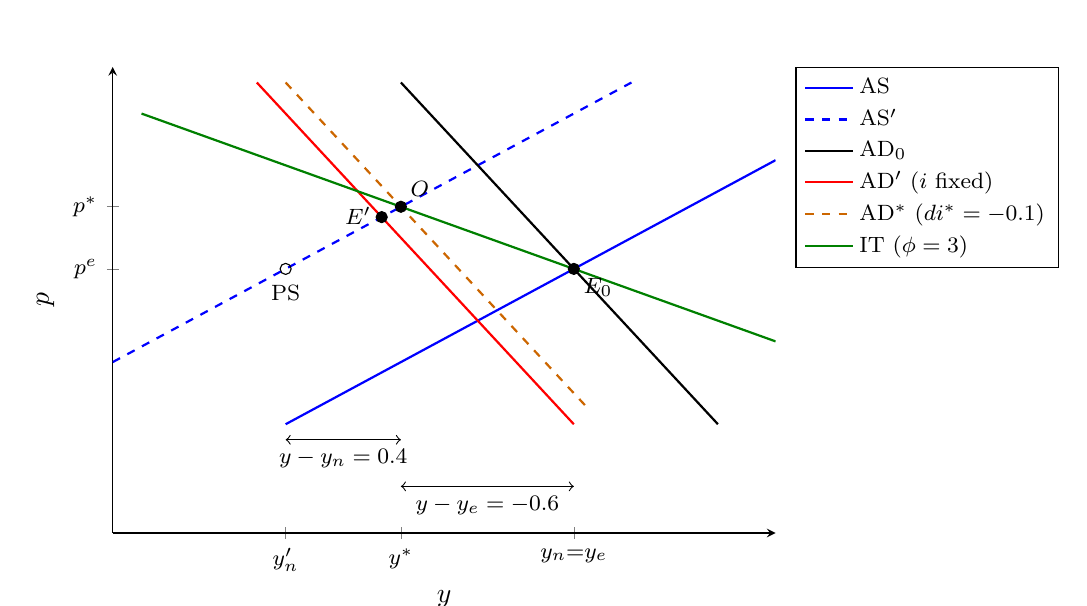
\begin{tikzpicture}
\begin{axis}[width=10cm,height=7.5cm,xmin=-1.6,xmax=0.7,ymin=-0.85,ymax=0.65,axis lines=left,xlabel={$y$},ylabel={$p$},
  xtick={-1,-0.6,0},xticklabels={$y_n'$,$y^*$,$y_n{=}y_e$},ytick={0,0.2},yticklabels={$p^e$,$p^*$},
  tick label style={font=\footnotesize},legend style={font=\footnotesize},legend pos=outer north east,legend cell align=left]
\addplot[thick,blue,domain=-1:0.7]{0.5*x};
\addplot[thick,blue,dashed,domain=-1.6:0.2]{0.5*(x+1)};
\addplot[thick,black,domain=-0.6:0.5]{-x};
\addplot[thick,red,domain=-1.1:0]{-(x+0.5)};
\addplot[thick,orange!80!black,dashed,domain=-1:0.05]{-(x+0.4)};
\addplot[thick,green!50!black,domain=-1.5:0.7]{-x/3};
\legend{AS,AS$'$,AD$_0$,AD$'$ ($i$ fixed),AD$^*$ ($di^*=-0.1$),IT ($\phi=3$)}
\addplot[only marks,mark=*] coordinates {(0,0) (-0.6667,0.1667) (-0.6,0.2)};
\addplot[only marks,mark=o] coordinates {(-1,0)};
\node[font=\footnotesize,anchor=north west] at (axis cs:0,0) {$E_0$};
\node[font=\footnotesize,anchor=east] at (axis cs:-0.67,0.17) {$E'$};
\node[font=\footnotesize,anchor=south west] at (axis cs:-0.6,0.2) {$O$};
\node[font=\footnotesize,anchor=north] at (axis cs:-1,-0.02) {PS};
\draw[<->] (axis cs:-1,-0.55) -- (axis cs:-0.6,-0.55) node[midway,below,font=\footnotesize]{$y-y_n=0.4$};
\draw[<->] (axis cs:-0.6,-0.7) -- (axis cs:0,-0.7) node[midway,below,font=\footnotesize]{$y-y_e=-0.6$};
\end{axis}
\end{tikzpicture}
\end{center}
\rubrica{\item Numbers: 1 pt. \item Graph (scored on its own): both AS, both AD, IT through $(y_e,p^e)$ with slope $-1/\phi$, $E_0$, $E'$, $O$, both gaps: 2 pts.}
\end{sol}

% -----------------------------------------------------------------------------
\questao{(10 points) \emph{Created.} Public spending rises by $\Delta>0$ in three ways: (i) temporarily, $dg=\Delta$, $d\bar g=0$; (ii) permanently,
$dg=d\bar g=\Delta$; (iii) as news only, $d\bar g=\Delta$, $dg=0$.}

\textbf{a)} (4 points) For each case: which curves move and by how much; $dy$, $dp$, $d(y-y_n)$ with $i$ fixed; and $d(y-y_e)$.
\resolespaco
\begin{sol}
\begin{notacao}
\item $y$, $p$, $\bar y$, $p^e$, $y_n$, $y_e$, $i$, $g$, $\bar g$, $\sigma>0$, $\eta>0$, $\kappa>0$, $\Omega\equiv\sigma^{-1}+\eta$: as in Question~1.
\item $\Delta>0$: the size of the spending rise. Cases (i) $dg=\Delta$, $d\bar g=0$; (ii) $dg=d\bar g=\Delta$; (iii) $dg=0$, $d\bar g=\Delta$.
\item $\phi\ge0$: weight in \eqref{LF}. $y^*$, $p^*$, $i^*$: optimal output, price and rate. $E_0$, $E'$: initial and no-policy points.
\end{notacao}
\passo{shifts}{Differentiate \eqref{YN} and \eqref{YE}:}
\begin{equation}
dy_n=dy_e=\frac{\sigma^{-1}}{\Omega}\,dg . \label{q10:dyn}
\end{equation}
So the AS shifts by $dy_n$. By \eqref{q1:dAD} and \eqref{YB}, the AD shifts by
\begin{equation}
d\bar y+dg-d\bar g=\Big(\frac{\sigma^{-1}}{\Omega}\,d\bar g\Big)+dg-d\bar g . \label{q10:ad}
\end{equation}
(i) AD $+\Delta$, AS $+\frac{\sigma^{-1}}{\Omega}\Delta$. (ii) AD $+\frac{\sigma^{-1}}{\Omega}\Delta$, AS $+\frac{\sigma^{-1}}{\Omega}\Delta$. (iii) using \eqref{q5:gb}, AD
$\big(\frac{\sigma^{-1}}{\Omega}-1\big)\Delta=-\frac{\eta}{\Omega}\Delta$, AS still. In all, \eqref{q10:dyn} gives $dy_e=dy_n$, so $d(y-y_e)=d(y-y_n)$.
\passo{(i)}{Put the shifts of (i) in \eqref{q1:M}, with $1-\frac{\sigma^{-1}}{\Omega}=\frac{\eta}{\Omega}$:}
\begin{align*}
(1+\sigma\kappa)\,d(y-y_n)&=(\Delta)-\Big(\frac{\sigma^{-1}}{\Omega}\Delta\Big)\\
&=\frac{\eta}{\Omega}\Delta .
\end{align*}
Divide by $1+\sigma\kappa$:
\begin{equation}
d(y-y_n)=\frac{\eta\Delta}{\Omega(1+\sigma\kappa)} . \label{q10:gap1}
\end{equation}
By \eqref{q1:dAS}, $dp=\kappa\,d(y-y_n)$; substitute \eqref{q10:gap1}:
\begin{align}
dp&=\kappa\Big(\frac{\eta\Delta}{\Omega(1+\sigma\kappa)}\Big)\nonumber\\
&=\frac{\kappa\eta\Delta}{\Omega(1+\sigma\kappa)} . \nonumber
\end{align}
Output is $dy=dy_n+d(y-y_n)$; use \eqref{q10:dyn} and \eqref{q10:gap1}:
\begin{align*}
dy&=\Big(\frac{\sigma^{-1}\Delta}{\Omega}\Big)+\Big(\frac{\eta\Delta}{\Omega(1+\sigma\kappa)}\Big)\\
&=\frac{(\sigma^{-1}+\kappa+\eta)\,\Delta}{\Omega(1+\sigma\kappa)}\\
&=\frac{(1+\kappa/\Omega)\,\Delta}{1+\sigma\kappa} .
\end{align*}
\passo{(ii)}{Put the shifts of (ii) in \eqref{q1:M}:}
\begin{equation}
(1+\sigma\kappa)\,d(y-y_n)=\Big(\frac{\sigma^{-1}}{\Omega}\Delta\Big)+(\Delta)-(\Delta)-\Big(\frac{\sigma^{-1}}{\Omega}\Delta\Big) . \nonumber
\end{equation}
Divide by $1+\sigma\kappa$:
\begin{equation}
d(y-y_n)=\frac{1}{1+\sigma\kappa}\Big(\frac{\sigma^{-1}}{\Omega}\Delta-\frac{\sigma^{-1}}{\Omega}\Delta\Big)=0 . \nonumber
\end{equation}
So $dp=0$ by \eqref{q1:dAS}, and $dy=dy_n=\frac{\sigma^{-1}\Delta}{\Omega}$ by \eqref{q10:dyn}.
\passo{(iii)}{Put the shifts of (iii) in \eqref{q1:M}:}
\begin{align}
(1+\sigma\kappa)\,d(y-y_n)&=\Big(\frac{\sigma^{-1}}{\Omega}\Delta\Big)-(\Delta)\nonumber\\
&=-\frac{\eta}{\Omega}\Delta . \nonumber
\end{align}
Divide by $1+\sigma\kappa$; $dy_n=0$, so output moves with the gap:
\begin{equation}
d(y-y_n)=dy=-\frac{\eta\Delta}{\Omega(1+\sigma\kappa)}<0 . \nonumber
\end{equation}
By \eqref{q1:dAS}, $dp=\kappa\,d(y-y_n)$; substitute the gap:
\begin{align}
dp&=\kappa\Big(-\frac{\eta\Delta}{\Omega(1+\sigma\kappa)}\Big)\nonumber\\
&=-\frac{\kappa\eta\Delta}{\Omega(1+\sigma\kappa)}<0 . \nonumber
\end{align}
\rubrica{\item Shifts, with $d\bar y-d\bar g=-\frac{\eta}{\Omega}d\bar g$: 1.5 pts. \item Three solutions: 2.5 pts ($-0.5$ per slip).}
\end{sol}

\textbf{b)} (3 points) Find the optimal $di^*$ in each case and show that $\phi$ does not enter. Check that (i) and (iii) add up to (ii).
\resolespaco
\begin{sol}
\begin{notacao}
\item Symbols as in (a). $X\equiv dy_e-dy_n$, as in Question 4(c).
\end{notacao}
\passo{rule}{By \eqref{q10:dyn}, $dy_n=dy_e$ in every case, so $X=0$ and \eqref{q4:ystar} gives $y^*=y_n=y_e$, $p^*=p^e$. Redo
\eqref{q4:di0}--\eqref{q4:di} with the AD shift $d\bar y+dg-d\bar g$ of \eqref{q1:dAD} in place of $d\bar y$, and set $X=0$:}
\begin{align}
di^*&=\frac{(d\bar y+dg-d\bar g)-(dy_n)}{\sigma}-\frac{(\sigma-\phi)\,\kappa\,(0)}{\sigma(1+\phi\kappa)}\nonumber\\
&=\frac{d\bar y+dg-d\bar g-dy_n}{\sigma} , \label{q10:di}
\end{align}
with no $\phi$.
\passo{cases}{Put \eqref{q10:ad} and \eqref{q10:dyn} in \eqref{q10:di}, case by case:}
\begin{align*}
\text{(i)}\quad di^*&=\frac{\Delta-\frac{\sigma^{-1}}{\Omega}\Delta}{\sigma}=\frac{\eta\Delta}{\sigma\Omega}\ \text{(raise)},\\
\text{(ii)}\quad di^*&=\frac{\frac{\sigma^{-1}}{\Omega}\Delta-\frac{\sigma^{-1}}{\Omega}\Delta}{\sigma}=0,\\
\text{(iii)}\quad di^*&=\frac{\frac{\sigma^{-1}}{\Omega}\Delta-\Delta}{\sigma}=-\frac{\eta\Delta}{\sigma\Omega}\ \text{(cut)}.
\end{align*}
Add (i) and (iii):
\begin{equation}
\frac{\eta\Delta}{\sigma\Omega}-\frac{\eta\Delta}{\sigma\Omega}=0 , \nonumber
\end{equation}
case (ii), by linearity.
\rubrica{\item Rule and $\phi$-independence: 1.5 pts. \item Three rates with signs and the sum: 1.5 pts.}
\end{sol}

\textbf{c)} (3 points) Draw the three diagrams for $\sigma=1$, $\eta=\kappa=0.5$, $\Delta=1.5$. Then, in words: what is the output multiplier when
the bank follows its optimal rule, and how does case (iii) relate to the $\bar\mu$ news of Prova 01?
\resolespaco
\begin{sol}
\begin{notacao}
\item Symbols as in (a). Values: $\sigma=1$, $\eta=\kappa=0.5$, $\Delta=1.5$. Output multiplier: $dy/\Delta$.
\end{notacao}
\passo{numbers}{The building blocks:}
\begin{align*}
\Omega&=1+0.5=1.5, & \tfrac{\sigma^{-1}}{\Omega}\Delta&=\tfrac{1.5}{1.5}=1,\\
\tfrac{\eta}{\Omega}\Delta&=\tfrac{0.75}{1.5}=0.5, & 1+\sigma\kappa&=1.5 .
\end{align*}
(i) By \eqref{q10:gap1}, $d(y-y_n)=\frac{0.5}{1.5}=\frac13$, so $dy=1+\frac13=\frac43$ and $dp=0.5\cdot\frac13=\frac16$: $E'=(\frac{4}{3},\frac16)$. The raise $\frac{\eta\Delta}{\sigma\Omega}=0.5$
moves it to $(1,0)$. (ii) $E'=(1,0)$. (iii) $dy=-\frac{0.5}{1.5}=-\frac13$, $dp=0.5\cdot(-\frac13)=-\frac16$: $E'=(-\frac13,-\frac16)$; the cut of $0.5$ brings it
back to $(0,0)$.
\begin{center}
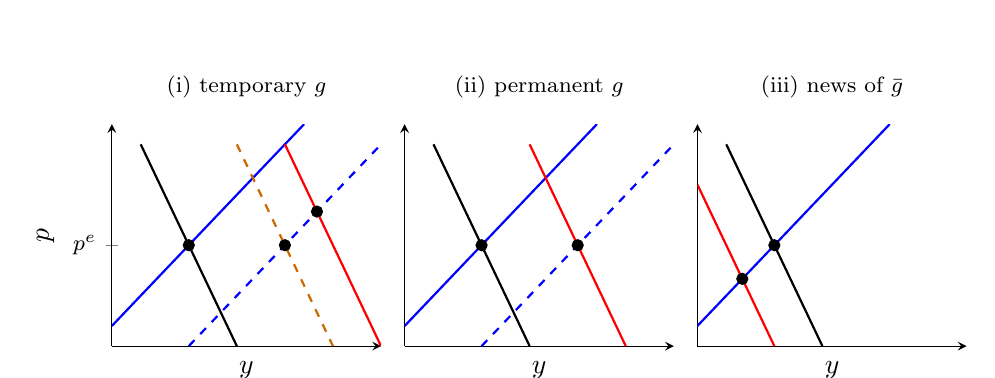
\begin{tikzpicture}
\begin{axis}[name=A,width=5cm,height=4.4cm,xmin=-0.8,xmax=2,ymin=-0.5,ymax=0.6,axis lines=left,xlabel={$y$},ylabel={$p$},
  xtick=\empty,ytick={0},yticklabels={$p^e$},title={\footnotesize (i) temporary $g$},tick label style={font=\footnotesize}]
\addplot[blue,thick,domain=-0.8:1.2]{0.5*x};\addplot[blue,thick,dashed,domain=0:2]{0.5*(x-1)};
\addplot[black,thick,domain=-0.5:0.5]{-x};\addplot[red,thick,domain=1:2]{-(x-1.5)};\addplot[orange!80!black,dashed,thick,domain=0.5:1.5]{-(x-1)};
\addplot[only marks,mark=*] coordinates {(0,0) (1.3333,0.1667) (1,0)};
\end{axis}
\begin{axis}[at={(A.east)},anchor=west,xshift=0.3cm,name=B,width=5cm,height=4.4cm,xmin=-0.8,xmax=2,ymin=-0.5,ymax=0.6,axis lines=left,
  xlabel={$y$},xtick=\empty,ytick=\empty,title={\footnotesize (ii) permanent $g$}]
\addplot[blue,thick,domain=-0.8:1.2]{0.5*x};\addplot[blue,thick,dashed,domain=0:2]{0.5*(x-1)};
\addplot[black,thick,domain=-0.5:0.5]{-x};\addplot[red,thick,domain=0.5:1.5]{-(x-1)};
\addplot[only marks,mark=*] coordinates {(0,0) (1,0)};
\end{axis}
\begin{axis}[at={(B.east)},anchor=west,xshift=0.3cm,width=5cm,height=4.4cm,xmin=-0.8,xmax=2,ymin=-0.5,ymax=0.6,axis lines=left,
  xlabel={$y$},xtick=\empty,ytick=\empty,title={\footnotesize (iii) news of $\bar g$}]
\addplot[blue,thick,domain=-0.8:1.2]{0.5*x};
\addplot[black,thick,domain=-0.5:0.5]{-x};\addplot[red,thick,domain=-0.8:0]{-(x+0.5)};
\addplot[only marks,mark=*] coordinates {(0,0) (-0.3333,-0.1667)};
\end{axis}
\end{tikzpicture}
\end{center}
{\footnotesize Blue: AS (dashed: AS$'$). Black: AD$_0$. Red: AD$'$ with $i$ fixed. Orange dashed: AD after the optimal raise in (i). In (iii) the optimal cut returns AD$'$ to AD$_0$.}
\passo{multiplier}{Under the optimal rule $y=y_n=y_e$ (part (b)), so by \eqref{q10:dyn}, in (i) and (ii), whatever the timing:}
\begin{equation}
\frac{dy}{\Delta}=\frac{\sigma^{-1}}{\Omega}=\frac{\sigma^{-1}}{\sigma^{-1}+\eta}=\frac{1}{1+\sigma\eta}<1 , \nonumber
\end{equation}
and $0$ in (iii), where $dg=0$.
The bank neutralises the demand part of fiscal policy; only its effect on capacity remains.
\passo{link to Prova 01}{(iii) is a pure AD shock from news about the long run, like $d\bar\mu>0$: AD left, AS still, prices and output fall, and
the optimal response is a cut, the same for every $\phi$.}
\refbib{Benigno (2015), \S8, Table 1, pp.~514--517; \S11, pp.~521--523.}
\rubrica{\item Graphs (scored on their own): shifts and equilibria in the three panels: 1.5 pts. \item Multiplier with the reason: 1 pt. \item Link: 0.5 pt.}
\end{sol}


\end{document}
